\documentclass[tikz]{tmr}

\title{Two Monoids for Approximating \np-Complete Problems}
\author{Mike Izbicki\email{mike@izbicki.me}}

\usepackage{rotating}

%%%%%%%%%%%%%%%%%%%%%%%%%%%%%%%%%%%%%%%
%% tikz settings

\usetikzlibrary{patterns}
\pgfdeclarepatternformonly{soft crosshatch}{\pgfqpoint{-1pt}{-1pt}}{\pgfqpoint{4pt}{4pt}}{\pgfqpoint{3pt}{3pt}}%
{
  \pgfsetstrokeopacity{0.3}
  \pgfsetlinewidth{0.4pt}
  \pgfpathmoveto{\pgfqpoint{3.1pt}{0pt}}
  \pgfpathlineto{\pgfqpoint{0pt}{3.1pt}}
  \pgfpathmoveto{\pgfqpoint{0pt}{0pt}}
  \pgfpathlineto{\pgfqpoint{3.1pt}{3.1pt}}
  \pgfusepath{stroke}
}

%%%%%%%%%%%%%%%%%%%%%%%%%%%%%%%%%%%%%%%
%% listings settings

\usepackage{listings}
\lstloadlanguages{Haskell}
\lstnewenvironment{spec}
    {}
    {}
\lstset{
    basicstyle=\small\ttfamily,
    xleftmargin=\parindent,
    xleftmargin=\parindent,
    flexiblecolumns=false,
    keepspaces=true,
    basewidth={0.5em,0.45em},
    literate={+}{{$+$}}1 {/}{{$/$}}1 {*}{{$*$}}1 {=}{{$=$}}1
            {>}{{$>$}}1 {<}{{$<$}}1 {\\}{{$\lambda$}}1
            {\\\\}{{\char`\\\char`\\}}1
            {->}{{$\rightarrow$}}2 {>=}{{$\geq$}}2 {<-}{{$\leftarrow$}}2
            {<=}{{$\leq$}}2 {=>}{{$\Rightarrow$}}2 
%                {\ .}{{$\circ$}}2 {\ .\ }{{$\circ$}}2
            {>>}{{>>}}2 {>>=}{{>>=}}2
            {|}{{$\mid$}}1               
            {<>}{{$\diamond$}}1          
            {++}{{$\+$}}1                
%             {mempty}{{$\epsilon$}}1               
%             {mappend}{{$\diamond$}}1               
}

\lstnewenvironment{code}
    {\lstset{
      numbers=left,
      firstnumber=1,
      numberfirstline=true
      }}
    {}
    
\newcommand\h{\lstinline}
     
%%%%%%%%%%%%%%%%%%%%%%%%%%%%%%%%%%%%%%%
% misc commands
    
\newcommand{\prob}[1]{{\sc {#1}}}
\newcommand{\np}{{\ensuremath{\mathbb{NP}}}}

\newcommand\doubleplus{+\kern-1.3ex+\kern0.8ex}
\newcommand\+{\mdoubleplus}
\newcommand\mdoubleplus{\ensuremath{\mathbin{+\mkern-10mu+}}}


\begin{document}

\begin{introduction}
As a TA I was confronted with a real life instance of the \np-complete \prob{Scheduling} problem.
To solve the problem, I turned to the classic Least Processing Time First (LPTF) approximation algorithm.
In this article, we'll see that because LPTF is a monoid homomorphism, we can implement it using HLearn's {\upshape\h{HomTrainer}} type class.
This gives us parallel and online versions of LPTF ``for free.''
We'll also be able to use these same techniques to solve a related problem called \prob{BinPacking}.
Hopefully, at the end of the article you'll understand when the {\upshape\h{HomTrainer}} class might be a useful tool, and how to use and build your own instances.
% What's more, LPTF is a particularly illustrative \h{HomTrainer} instance for three reasons.
% First, the monoid operation for \prob{Scheduling} takes non-constant time, and the \h{HomTrainer} class makes reasoning about this run time straightforward.
% Second, the monoid uses lazy semantics to improve performance.  
% Finally, it demonstrates the versatility of the \h{HomTrainer} to domains outside of machine learning.
\end{introduction}

\section{Framing The Problem}
I enjoy TAing the introduction to C++ course at my university.
Teaching pointer arithmetic can be immensely frustrating, but it's worth it to see the students when it all finally clicks.  
% (
% (Not to mention the subtle indoctrination against these low level languages.)
% Of course, watching them struggle for hours to hunt down a segfault reminds me why Haskell is so awesome.
% I enjoy teaching.  
% It's really fun helping my intro to C++ students struggle through pointer arithmetic.  
% (I doubt the students feel the same way after spending five hours tracking down a segfault!)
%(It's only fun because \emph{I} am not the one spending hours tracking down the segfaults!)
% Ah, the joys of segfaults... 
%(to be young and segfaulting...)
Teaching is even better when it causes you to stumble onto an interesting problem.  
Oddly enough, I found this cool Haskell problem because of my C++ teaching assistanceship.

The professor wanted to assign a group project, and I had to pick the groups.
There had to be exactly five groups, and the groups needed to be as fair as possible.
% The only requirement was that the groups should be as fair as possible.
%He didn't want to let students pick their own groups because he wanted the groups to be as fair as possible.
In other words, I was supposed to evenly distribute the best and worst students.
% Because of this fairness criterion, I couldn't let the students pick their own groups.
% Because of these requirements, the students couldn't pick their own groups.

After a little thought, I realized this was an instance of the \np-complete \prob{Scheduling} problem in disguise.
This problem was first formulated in the context of concurrent computing.
In the textbook example of \prob{Scheduling}, we are given $p$ processors and $n$ tasks.
Each task $t_i$ has some associated time it will take to complete it.
The goal is to assign the tasks to processors so as to complete the tasks as quickly as possible.

The \prob{Scheduling} problem is shown graphically in Figure \ref{fig:scheduling}.
Processors are drawn as bins (labeled $b_1 ... b_4$), and tasks are drawn as green blocks (labeled $t_1 ... t_{10}$) and placed inside a bin.
The height of the task $t_i$ represents the length of time required to process that task.
Our goal is to minimize the \textcolor{red}{red} processing time.

\begin{figure}[H]
\centering
\caption{The \prob{Scheduling} problem}
\label{fig:scheduling}
\resizebox{!}{2in}{
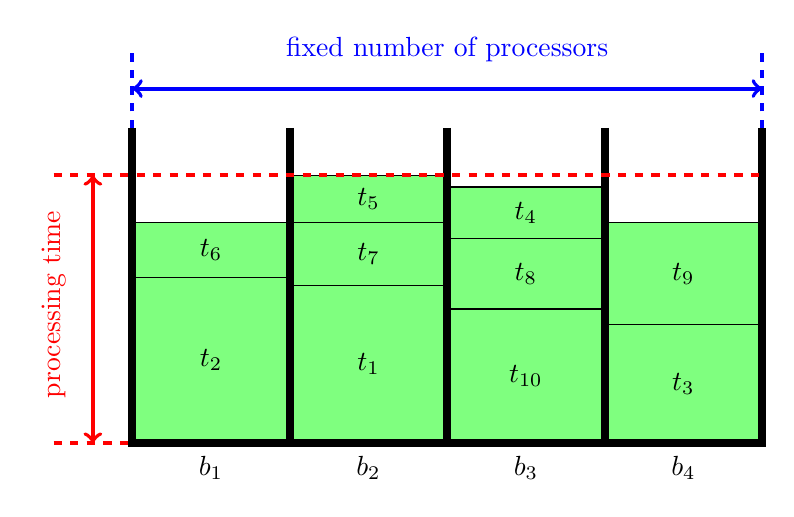
\begin{tikzpicture}
\definecolor{hlearn_bgbox}{RGB}{127,255,127}
\node[shape=rectangle,draw,fill=hlearn_bgbox,minimum width=2cm,minimum height=2.1cm] at (3,1.05) { $t_{2}$ };
\node[shape=rectangle,draw,fill=hlearn_bgbox,minimum width=2cm,minimum height=0.7cm] at (3,2.45) { $t_{6}$ };
\node[shape=rectangle,draw,fill=hlearn_bgbox,minimum width=2cm,minimum height=2.0cm] at (5,1.0) { $t_{1}$ };
\node[shape=rectangle,draw,fill=hlearn_bgbox,minimum width=2cm,minimum height=0.8cm] at (5,2.4) { $t_{7}$ };
\node[shape=rectangle,draw,fill=hlearn_bgbox,minimum width=2cm,minimum height=0.6cm] at (5,3.0999999999999996) { $t_{5}$ };
\node[shape=rectangle,draw,fill=hlearn_bgbox,minimum width=2cm,minimum height=1.7cm] at (7,0.85) { $t_{10}$ };
\node[shape=rectangle,draw,fill=hlearn_bgbox,minimum width=2cm,minimum height=0.9cm] at (7,2.15) { $t_{8}$ };
\node[shape=rectangle,draw,fill=hlearn_bgbox,minimum width=2cm,minimum height=0.65cm] at (7,2.9250000000000003) { $t_{4}$ };
\node[shape=rectangle,draw,fill=hlearn_bgbox,minimum width=2cm,minimum height=1.5cm] at (9,0.75) { $t_{3}$ };
\node[shape=rectangle,draw,fill=hlearn_bgbox,minimum width=2cm,minimum height=1.3cm] at (9,2.15) { $t_{9}$ };
\draw[line width=0.1cm] (2,4) to (2,0) to node[below] {$b_{1}$} (2+2,0) to (2+2,4);
\draw[line width=0.1cm] (4,4) to (4,0) to node[below] {$b_{2}$} (4+2,0) to (4+2,4);
\draw[line width=0.1cm] (6,4) to (6,0) to node[below] {$b_{3}$} (6+2,0) to (6+2,4);
\draw[line width=0.1cm] (8,4) to (8,0) to node[below] {$b_{4}$} (8+2,0) to (8+2,4);

\draw[dashed,color=red,line width=0.05cm] (1,3.4) to (10,3.4);
\draw[dashed,color=red,line width=0.05cm] (1,0) to (2,0);
\draw[<->,color=red,line width=0.05cm] (1.5,3.4) to  (1.5,0);
\node[color=red] at (1,1.7) {\rotatebox{90}{
    \begin{tabular}{c}
%     variable\\
    processing time
    \end{tabular}}};
\draw[dashed,color=blue,line width=0.05cm] (2,4) to (2,5);
\draw[dashed,color=blue,line width=0.05cm] (10,4) to (10,5);
\draw[<->,color=blue,line width = 0.05cm] (2,4.5) to (10,4.5);
\node[color=blue] at (6,5) {fixed number of processors};
\end{tikzpicture}
}
\vspace{0.1in}
\end{figure}

What does this have to do with the problem my professor gave me?
Well, we can think of the number of groups as the number of processors, each student is a task, and the student's current grade is the task's processing time.
Then, the problem is to find a way to divvy up the students so that the sum of grades for the ``best'' group is as small as possible.
We'll see some code for solving this problem in a bit.

There is another closely related problem called \prob{BinPacking} that is easily confused with \prob{Scheduling}.
In \prob{BinPacking}, instead of fixing the number of bins and minimizing the amount in the bins, we fix the capacity of each bin and minimize the total number of bins used.
Compare Figure \ref{fig:binpacking} below and Figure \ref{fig:scheduling} above to see the difference.
The \prob{BinPacking} problem was originally studied by shipping companies, although like \prob{Sheduling} it occurs in many domains.
% The original motivation for the \prob{BinPacking} problem was in shipping.
% Every container shipped costs the same amount, no matter how much is stored in side of it.
% Therefore, we would like to reduce the number of containers we use to ship our products.

\begin{figure}[H]
\caption{The \prob{BinPacking} problem}
\label{fig:binpacking}
\centering
\resizebox{!}{1.5in}{
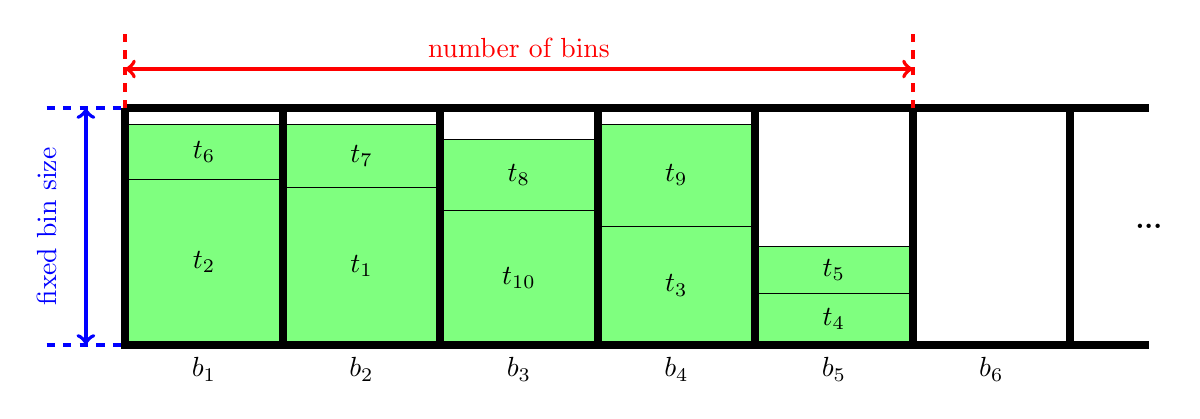
\begin{tikzpicture}
\definecolor{hlearn_bgbox}{RGB}{127,255,127}
\node[shape=rectangle,draw,fill=hlearn_bgbox,minimum width=2cm,minimum height=2.1cm] at (3,1.05) { $t_{2}$ };
\node[shape=rectangle,draw,fill=hlearn_bgbox,minimum width=2cm,minimum height=0.7cm] at (3,2.45) { $t_{6}$ };
\node[shape=rectangle,draw,fill=hlearn_bgbox,minimum width=2cm,minimum height=2.0cm] at (5,1.0) { $t_{1}$ };
\node[shape=rectangle,draw,fill=hlearn_bgbox,minimum width=2cm,minimum height=0.8cm] at (5,2.4) { $t_{7}$ };
\node[shape=rectangle,draw,fill=hlearn_bgbox,minimum width=2cm,minimum height=1.7cm] at (7,0.85) { $t_{10}$ };
\node[shape=rectangle,draw,fill=hlearn_bgbox,minimum width=2cm,minimum height=0.9cm] at (7,2.15) { $t_{8}$ };
\node[shape=rectangle,draw,fill=hlearn_bgbox,minimum width=2cm,minimum height=1.5cm] at (9,0.75) { $t_{3}$ };
\node[shape=rectangle,draw,fill=hlearn_bgbox,minimum width=2cm,minimum height=1.3cm] at (9,2.15) { $t_{9}$ };
\node[shape=rectangle,draw,fill=hlearn_bgbox,minimum width=2cm,minimum height=0.65cm] at (11,0.325) { $t_{4}$ };
\node[shape=rectangle,draw,fill=hlearn_bgbox,minimum width=2cm,minimum height=0.6cm] at (11,0.95) { $t_{5}$ };
\draw[line width=0.1cm] (2,3.0) to (2,0) to node[below] {$b_{1}$} (2+2,0) to (2+2,3.0);
\draw[line width=0.1cm] (4,3.0) to (4,0) to node[below] {$b_{2}$} (4+2,0) to (4+2,3.0);
\draw[line width=0.1cm] (6,3.0) to (6,0) to node[below] {$b_{3}$} (6+2,0) to (6+2,3.0);
\draw[line width=0.1cm] (8,3.0) to (8,0) to node[below] {$b_{4}$} (8+2,0) to (8+2,3.0);
\draw[line width=0.1cm] (10,3.0) to (10,0) to node[below] {$b_{5}$} (10+2,0) to (10+2,3.0);
\draw[line width=0.1cm] (12,3.0) to (12,0) to node[below] {$b_{6}$} (12+2,0) to (12+2,3.0);
% \draw[line width=0.1cm] (14,3.0) to (14,0) to node[below] {$b_{5}$} (14+2,0) to (14+2,3.0);
% \draw[line width=0.1cm] (16,3.0) to (16,0) to node[below] {$b_{5}$} (16+2,0) to (16+2,3.0);
\draw[line width=0.1cm] (2,3.0) to (15,3.0);
\draw[line width=0.1cm] (2,0) to (15,0);
\draw[dashed,color=red,line width=0.05cm] (2,3) to (2,4);
\draw[dashed,color=red,line width=0.05cm] (12,3) to (12,4);
\draw[<->,line width=0.05cm,color=red] (2,3.5) to node[above] {number of bins} (12,3.5);
\draw[<->,line width=0.05cm,color=blue] (1.5,0) to (1.5,3);
\draw[dashed,color=blue,line width=0.05cm] (1,0) to (2,0);
\draw[dashed,color=blue,line width=0.05cm] (1,3) to (2,3);
\node[color=blue] at (1,1.5) {\rotatebox{90}{fixed bin size}};
\node at (15,1.5) {\textbf{...}};
\end{tikzpicture}
}
\end{figure}

Both \prob{Scheduling} and \prob{BinPacking} are \np-complete.
% Since \prob{Scheduling} is \np-complete, finding an exact solution takes exponential time.  
Therefore, I had no chance of creating an optimal grouping for my professor---the class had 100 students, and $2^{100}$ is a \textit{big} number!
So I turned to approximation algorithms.
% These algorithms give us solutions that are guaranteed to be within a certain factor of optimal.
One popular approximation for \prob{Scheduling} is called Longest Processing Time First (LPTF).
When analyzing these approximation algorithms, it is customary to compare the quality of their result with that of the theoretical optimal result.
% Even when it is impractical to actually calculate this optimal, we can often bound it to within a certain range.
In this case, we denote the total processing time of the schedule returned by LPTF as \textit{LPTF}, and the processing time of the optimal solution as \textit{OPT}.
It can be shown that the following bound holds:
$$
\textit{LPTF} \le \left( {4\over3} - {1\over{3n}} \right) \textit{OPT}
$$
This bound was proven in the late 1960's, but the original paper remains quite readable today \cite{graham69}.
% For a survey on variants of the Scheduling problem, see Chapter 1 of \textit{Approximation Algorithms for NP Hard Problems} \cite{hochbaum96scheduling}.
By making this small sacrifice in accuracy, we get an algorithm that runs in time $\Theta(n\log n)$ instead of $\Theta(2^n)$.  Much better!  In the rest of this article, we'll take a detailed look at a Haskell implementation of the LPTF algorithm, and then briefly use similar techniques to solve the \prob{BinPacking} problem.

\section{The Scheduling HomTrainer}

When implementing an algorithm in Haskell, you always start with the type signature.
% I set out to implement the LPTF algorithm, and like all good Haskellers I started with the type signature.
LPTF takes a collection of tasks and produces a schedule, so it's type might look something like:
\begin{spec}
:: [Task] -> Schedule
\end{spec}
Anytime I see see a function of this form, I ask myself, ``Can it be implemented using the \h{HomTrainer} type class?''
\h{HomTrainer}s are useful because the compiler automatically derives online and parallel algorithms for all instances.
For LPTF, the answer is ``yes.''
This section will cover what exactly that means.

We start by looking at the format of a \h{HomTrainer} instance as shown graphically in Figure \ref{fig:HomTrainer} below.

\begin{figure}[H]
\caption{Basic requirements of the HomTrainer type class}
\label{fig:HomTrainer}
\centering
\tikzstyle{blackbox}=[shape=rectangle, draw, fill=black, text=white, minimum width=0.8in]
\definecolor{darkgreen}{RGB}{0,127,0}
\begin{tikzpicture}%[node distance=2.5in, auto, >=stealth]
\node[blackbox] (dataset) [minimum height=0.3in] {\textbf{data set}};
\node[blackbox] (model)   [minimum height=0.3in, node distance=2in,right of = dataset] {\textbf{model}};
\node[blackbox] (answer)  [minimum height=0.3in, node distance=2in,right of = model] {\textbf{answer}};
\draw[->,ultra thick] (dataset) to node[above] {train} (model);
\draw[->,ultra thick] (model) to node[above] {question} (answer);

\node (l1) [color=blue] at (-0.1,-1.3) {free monoid};
\node (l2) [color=blue] at (2.5,1.5) {homomorphism};
\node (l3) [color=blue] at (5.5,-1.3) {monoid};
\node (l4) [color=darkgreen] at (5.5,1.3) {\h{HomTrainer}};

\draw[->,color=blue,ultra thick] (l1) to (dataset);
\draw[->,color=blue,ultra thick] (l2) to (2.5,0.5);
\draw[->,color=blue,ultra thick] (l3) to (model);
\draw[->,color=darkgreen,ultra thick] (l4) to (model);
\end{tikzpicture}
\vspace{0.15in}
\end{figure}

There's a lot going on in Figure \ref{fig:HomTrainer}, but we'll look at things piece-by-piece.
The black boxes represent data types and the black arrows represent functions.
In our case, the data set is the collection of tasks we want scheduled and the model is the schedule.
The train function is the LPTF algorithm, which generates a model from the data points.
Finally, our model is only useful if we can ask it questions.
In this case, we might want to ask, ``Which processor is assigned to task $t_{10}$?'' or ``What are all the tasks assigned to processor 2?''
% The answer type would be a processor.
% This framework was originally meant for use with machine learning algorithms, however it is general enough to be applied in many contexts.

The blue arrows in the diagram are a little trickier.
They specify that our training algorithm must be a \emph{monoid homomorphism} from the \emph{free monoid}.
% This sounds a lot scarier than it actually is.
These are scary sounding words, but they're pretty simple once you're familiar with them.
We'll define them and see some examples.

In Haskell, the \h{Monoid} type class is defined as having an identity called \h{mempty} and a binary operation called \h{mappend}:
\begin{spec}
class Monoid m where
    mempty  :: m
    mappend :: m -> m -> m
\end{spec}
Sometimes we use the infix operation \h{(<>) = mappend} to make our code easier to read.
All instances must obey the identity and associativity laws:
\begin{spec}
mempty <> m = m <> mempty = m
(m1 <> m2) <> m3 = m1 <> (m2 <> m3)
\end{spec}
% \end{spec}
% mappend mempty m = mappend m mempty = m
% and associativity law:
% \begin{spec}
% $$
% \epsilon \diamond m = m\diamond \epsilon = m
% $$
Lists are one of the simplest examples of monoids.
Their identity element is the empty list, and their binary operation is concatenation:
\begin{spec}
instance Monoid [a] where
    mempty = []
    mappend = ++
\end{spec}
Vectors have a similar definition, and both lists and vectors are examples of free monoids.
Free monoids are monoids that can be generated by some underlying set.
In our monoid instance for lists above, the underlying set is the type variable \h{a}.
For the \h{HomTrainer}, when we say that our data set must be a free monoid, all we mean is that it is a collection of some data points
(\eg\ a list of tasks).

A homomorphism from the free monoid is a function that ``preserves the free monoid's structure.''
More formally, if the function is called \h{train}, then it obeys the law that for all \lstinline{xs} and \lstinline{ys} of type \lstinline{[a]}:
\begin{spec}
train (xs ++ ys) = (train xs) <> (train ys)
\end{spec}
The LPTF algorithm turns out to have this property.
Figure \ref{fig:LPTF-monoid} shows this in picture form with a commutative diagram.
This means that it doesn't matter whether we take the orange path (first train schedules from our data sets, then combine the schedules with \h{mappend}) or the purple path (first concatenate our data sets, then train a schedule on the result).
Either way, we get the exact same answer.

\begin{figure}[H]
\caption{The LPTF is a monoid homomorphism because this diagram commutes}
\label{fig:LPTF-monoid}
% \centering
\hspace{-0.3in}
\begin{tikzpicture}

\draw[->,line width=0.05cm,color=orange] (-2in,3.3) to (-2in,2.5);
\draw[->,line width=0.05cm,color=orange] (0in,3.3) to (0in,2.5);
\draw[dotted,line width=0.025cm,color=orange] (-2in,2.5) to (-2in,-2.5);
\draw[dotted,line width=0.025cm,color=orange] (0in,2.5) to (0in,-2.5);
\draw[->,line width=0.05cm,color=orange] (0in,-2.5) to (0in,-3) to (2.5in,-3) to (2.5in,-2.5);
\draw[->,line width=0.05cm,color=orange] (-2in,-2.5) to (-2in,-3) to (2.5in,-3) to (2.5in,-2.5);
\draw[->,line width=0.05cm,color=purple]  (2.5in,3.3) to (2.5in,2.5);
\draw[->,line width=0.05cm,color=purple] (0in,4.8) to (0in,5.3) to (2.5in,5.3) to (2.5in,4.8);
\draw[->,line width=0.05cm,color=purple] (-2in,4.8) to (-2in,5.3) to (2.5in,5.3) to (2.5in,4.8);
\draw[dotted,line width=0.025cm,color=purple] (2.5in,4.8) to (2.5in,3.3);


\node at (-2in,4) {
    \resizebox{!}{0.25in}{
    \begin{tikzpicture}
    \definecolor{hlearn_bgbox}{RGB}{127,255,127}
    \definecolor{hlearn_bgboxB}{RGB}{224,224,255}
    \node[shape=rectangle,draw,fill=hlearn_bgbox,minimum width=2cm,minimum height=2.1cm]   at (1,1.05) { $t_{a,1}$ };
    \node[shape=rectangle,draw,fill=hlearn_bgbox,minimum width=2cm,minimum height=2.7cm]   at (3,1.35) { $t_{a,2}$ };
    \node[shape=rectangle,draw,fill=hlearn_bgbox,minimum width=2cm,minimum height=3.1cm]   at (5,1.55) { $t_{a,3}$ };;
    \node[shape=rectangle,draw,fill=hlearn_bgbox,minimum width=2cm,minimum height=1.7cm]   at (7,0.85) { $t_{a,4}$ };
    \node[shape=rectangle,draw,fill=hlearn_bgbox,minimum width=2cm,minimum height=1.6cm]   at (9,0.8) { $t_{a,5}$ };
    \node[shape=rectangle,draw,fill=hlearn_bgbox,minimum width=2cm,minimum height=0.6cm]   at (11,0.3) { $t_{a,6}$ };
    \end{tikzpicture}
    }};

\node at (-2in,0) {
    \resizebox{1.5in}{!}{
    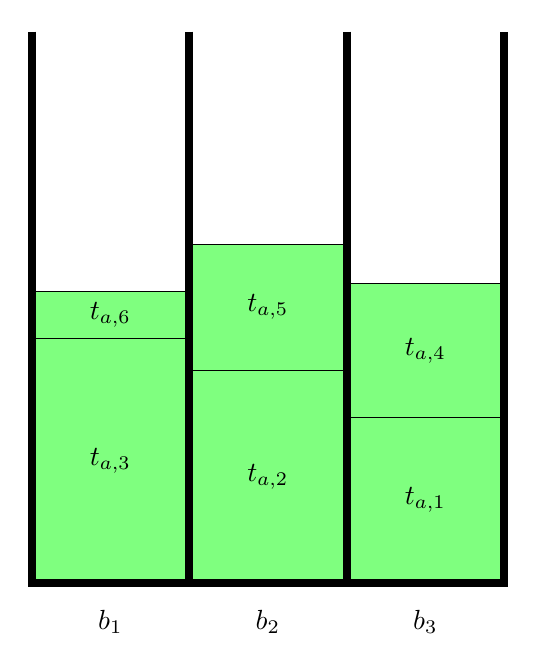
\begin{tikzpicture}
    \definecolor{hlearn_bgbox}{RGB}{127,255,127}
    \node[shape=rectangle,draw,fill=hlearn_bgbox,minimum width=2cm,minimum height=3.1cm] at (3,1.55) { $t_{a,3}$ };
    \node[shape=rectangle,draw,fill=hlearn_bgbox,minimum width=2cm,minimum height=0.6cm] at (3,3.4) { $t_{a,6}$ };
    \node[shape=rectangle,draw,fill=hlearn_bgbox,minimum width=2cm,minimum height=2.7cm] at (5,1.35) { $t_{a,2}$ };
    \node[shape=rectangle,draw,fill=hlearn_bgbox,minimum width=2cm,minimum height=1.6cm] at (5,3.5) { $t_{a,5}$ };
    \node[shape=rectangle,draw,fill=hlearn_bgbox,minimum width=2cm,minimum height=2.1cm] at (7,1.05) { $t_{a,1}$ };
    \node[shape=rectangle,draw,fill=hlearn_bgbox,minimum width=2cm,minimum height=1.7cm] at (7,2.95) { $t_{a,4}$ };
    \draw[line width=0.1cm] (2,7.0) to (2,0) to (2+2,0) to (2+2,7.0);
    \draw[line width=0.1cm] (4,7.0) to (4,0) to (4+2,0) to (4+2,7.0);
    \draw[line width=0.1cm] (6,7.0) to (6,0) to (6+2,0) to (6+2,7.0);
    \node at (3,-0.5) {$b_{1}$};
    \node at (5,-0.5) {$b_{2}$};
    \node at (7,-0.5) {$b_{3}$};
    \end{tikzpicture}
    }};

\node at (0,4) {
    \resizebox{!}{0.25in}{
%     \resizebox{1.75in}{!}{
    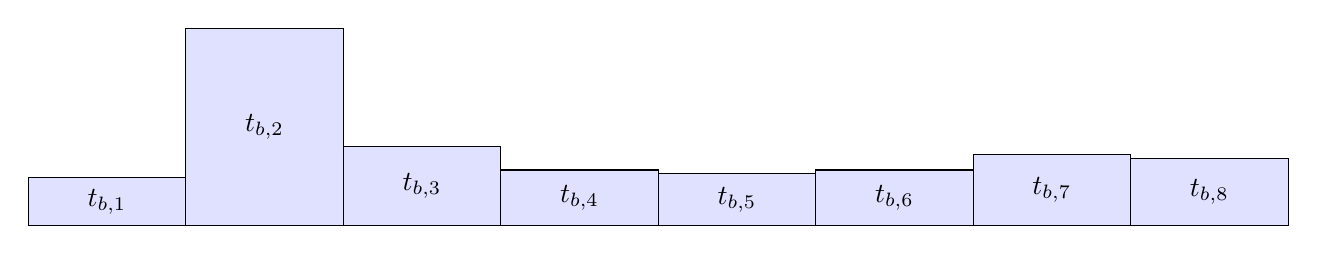
\begin{tikzpicture}
    \definecolor{hlearn_bgbox}{RGB}{127,255,127}
    \definecolor{hlearn_bgboxB}{RGB}{224,224,255}
    \node[shape=rectangle,draw,fill=hlearn_bgboxB,minimum width=2cm,minimum height=0.6cm]  at (1,0.3) { $t_{b,1}$ };
    \node[shape=rectangle,draw,fill=hlearn_bgboxB,minimum width=2cm,minimum height=2.5cm]  at (3,1.25) { $t_{b,2}$ };
    \node[shape=rectangle,draw,fill=hlearn_bgboxB,minimum width=2cm,minimum height=1.0cm]  at (5,0.5) { $t_{b,3}$ };
    \node[shape=rectangle,draw,fill=hlearn_bgboxB,minimum width=2cm,minimum height=0.7cm]  at (7,0.35) { $t_{b,4}$ };
    \node[shape=rectangle,draw,fill=hlearn_bgboxB,minimum width=2cm,minimum height=0.65cm] at (9,0.325) { $t_{b,5}$ };
    \node[shape=rectangle,draw,fill=hlearn_bgboxB,minimum width=2cm,minimum height=0.7cm]  at (11,0.35) { $t_{b,6}$ };
    \node[shape=rectangle,draw,fill=hlearn_bgboxB,minimum width=2cm,minimum height=0.9cm]  at (13,0.45) { $t_{b,7}$ };
    \node[shape=rectangle,draw,fill=hlearn_bgboxB,minimum width=2cm,minimum height=0.85cm] at (15,0.425) { $t_{b,8}$ };
    \end{tikzpicture}
    }};

\node at (0,0) {
    \resizebox{1.5in}{!}{
    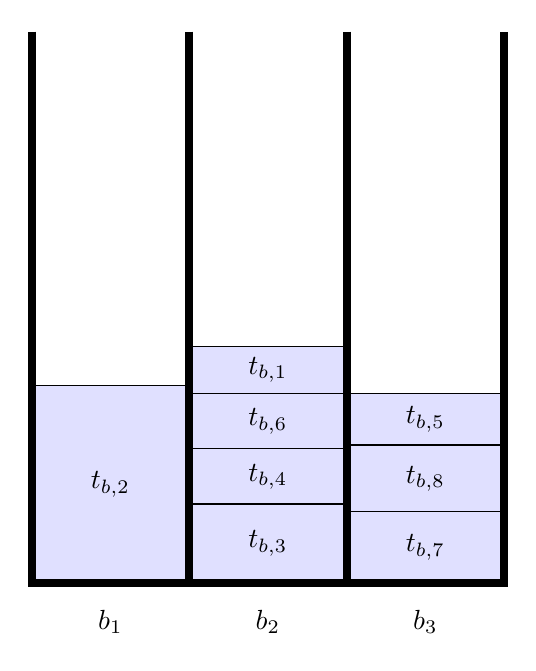
\begin{tikzpicture}
    \definecolor{hlearn_bgboxB}{RGB}{224,224,255}
    \node[shape=rectangle,draw,fill=hlearn_bgboxB,minimum width=2cm,minimum height=2.5cm] at (3,1.25) { $t_{b,2}$ };
    \node[shape=rectangle,draw,fill=hlearn_bgboxB,minimum width=2cm,minimum height=1.0cm] at (5,0.5) { $t_{b,3}$ };
    \node[shape=rectangle,draw,fill=hlearn_bgboxB,minimum width=2cm,minimum height=0.7cm] at (5,1.35) { $t_{b,4}$ };
    \node[shape=rectangle,draw,fill=hlearn_bgboxB,minimum width=2cm,minimum height=0.7cm] at (5,2.05) { $t_{b,6}$ };
    \node[shape=rectangle,draw,fill=hlearn_bgboxB,minimum width=2cm,minimum height=0.6cm] at (5,2.6999999999999997) { $t_{b,1}$ };
    \node[shape=rectangle,draw,fill=hlearn_bgboxB,minimum width=2cm,minimum height=0.9cm] at (7,0.45) { $t_{b,7}$ };
    \node[shape=rectangle,draw,fill=hlearn_bgboxB,minimum width=2cm,minimum height=0.85cm] at (7,1.325) { $t_{b,8}$ };
    \node[shape=rectangle,draw,fill=hlearn_bgboxB,minimum width=2cm,minimum height=0.65cm] at (7,2.075) { $t_{b,5}$ };
    \draw[line width=0.1cm] (2,7.0) to (2,0) to (2+2,0) to (2+2,7.0);
    \draw[line width=0.1cm] (4,7.0) to (4,0) to (4+2,0) to (4+2,7.0);
    \draw[line width=0.1cm] (6,7.0) to (6,0) to (6+2,0) to (6+2,7.0);
    \node at (3,-0.5) {$b_{1}$};
    \node at (5,-0.5) {$b_{2}$};
    \node at (7,-0.5) {$b_{3}$};
    \end{tikzpicture}
    }};

\node at (2.5in,4) {
    \resizebox{!}{0.25in}{
    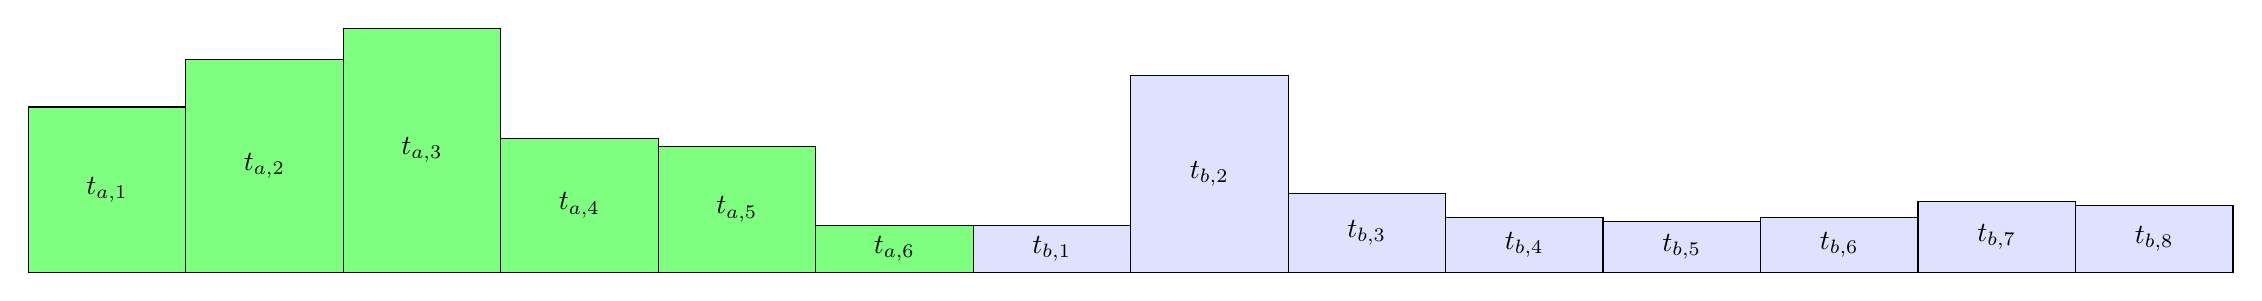
\begin{tikzpicture}
    \definecolor{hlearn_bgbox}{RGB}{127,255,127}
    \definecolor{hlearn_bgboxB}{RGB}{224,224,255}
    \node[shape=rectangle,draw,fill=hlearn_bgbox,minimum width=2cm,minimum height=2.1cm]   at (1,1.05) { $t_{a,1}$ };
    \node[shape=rectangle,draw,fill=hlearn_bgbox,minimum width=2cm,minimum height=2.7cm]   at (3,1.35) { $t_{a,2}$ };
    \node[shape=rectangle,draw,fill=hlearn_bgbox,minimum width=2cm,minimum height=3.1cm]   at (5,1.55) { $t_{a,3}$ };;
    \node[shape=rectangle,draw,fill=hlearn_bgbox,minimum width=2cm,minimum height=1.7cm]   at (7,0.85) { $t_{a,4}$ };
    \node[shape=rectangle,draw,fill=hlearn_bgbox,minimum width=2cm,minimum height=1.6cm]   at (9,0.8) { $t_{a,5}$ };
    \node[shape=rectangle,draw,fill=hlearn_bgbox,minimum width=2cm,minimum height=0.6cm]   at (11,0.3) { $t_{a,6}$ };
    \node[shape=rectangle,draw,fill=hlearn_bgboxB,minimum width=2cm,minimum height=0.6cm]  at (13,0.3) { $t_{b,1}$ };
    \node[shape=rectangle,draw,fill=hlearn_bgboxB,minimum width=2cm,minimum height=2.5cm]  at (15,1.25) { $t_{b,2}$ };
    \node[shape=rectangle,draw,fill=hlearn_bgboxB,minimum width=2cm,minimum height=1.0cm]  at (17,0.5) { $t_{b,3}$ };
    \node[shape=rectangle,draw,fill=hlearn_bgboxB,minimum width=2cm,minimum height=0.7cm]  at (19,0.35) { $t_{b,4}$ };
    \node[shape=rectangle,draw,fill=hlearn_bgboxB,minimum width=2cm,minimum height=0.65cm] at (21,0.325) { $t_{b,5}$ };
    \node[shape=rectangle,draw,fill=hlearn_bgboxB,minimum width=2cm,minimum height=0.7cm]  at (23,0.35) { $t_{b,6}$ };
    \node[shape=rectangle,draw,fill=hlearn_bgboxB,minimum width=2cm,minimum height=0.9cm]  at (25,0.45) { $t_{b,7}$ };
    \node[shape=rectangle,draw,fill=hlearn_bgboxB,minimum width=2cm,minimum height=0.85cm] at (27,0.425) { $t_{b,8}$ };
    \end{tikzpicture}
    }};

\node at (2.5in,0) {
    \resizebox{1.5in}{!}{
    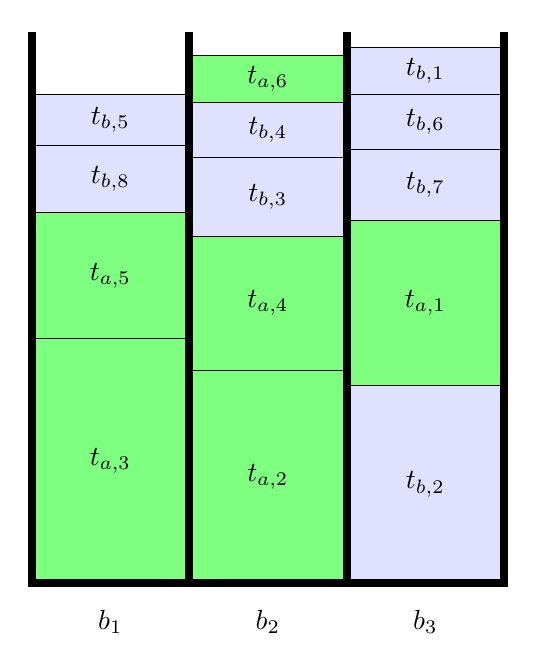
\begin{tikzpicture}
    \definecolor{hlearn_bgbox}{RGB}{127,255,127}
    \definecolor{hlearn_bgboxB}{RGB}{224,224,255}
    \node[shape=rectangle,draw,fill=hlearn_bgbox,minimum width=2cm,minimum height=3.1cm] at (3,1.55) { $t_{a,3}$ };
    \node[shape=rectangle,draw,fill=hlearn_bgbox,minimum width=2cm,minimum height=1.6cm] at (3,3.9000000000000004) { $t_{a,5}$ };
    \node[shape=rectangle,draw,fill=hlearn_bgboxB,minimum width=2cm,minimum height=0.85cm] at (3,5.125) { $t_{b,8}$ };
    \node[shape=rectangle,draw,fill=hlearn_bgboxB,minimum width=2cm,minimum height=0.65cm] at (3,5.875) { $t_{b,5}$ };
    \node[shape=rectangle,draw,fill=hlearn_bgbox,minimum width=2cm,minimum height=2.7cm] at (5,1.35) { $t_{a,2}$ };
    \node[shape=rectangle,draw,fill=hlearn_bgbox,minimum width=2cm,minimum height=1.7cm] at (5,3.5500000000000003) { $t_{a,4}$ };
    \node[shape=rectangle,draw,fill=hlearn_bgboxB,minimum width=2cm,minimum height=1.0cm] at (5,4.9) { $t_{b,3}$ };
    \node[shape=rectangle,draw,fill=hlearn_bgboxB,minimum width=2cm,minimum height=0.7cm] at (5,5.75) { $t_{b,4}$ };
    \node[shape=rectangle,draw,fill=hlearn_bgbox,minimum width=2cm,minimum height=0.6cm] at (5,6.4) { $t_{a,6}$ };
    \node[shape=rectangle,draw,fill=hlearn_bgboxB,minimum width=2cm,minimum height=2.5cm] at (7,1.25) { $t_{b,2}$ };
    \node[shape=rectangle,draw,fill=hlearn_bgbox,minimum width=2cm,minimum height=2.1cm] at (7,3.55) { $t_{a,1}$ };
    \node[shape=rectangle,draw,fill=hlearn_bgboxB,minimum width=2cm,minimum height=0.9cm] at (7,5.05) { $t_{b,7}$ };
    \node[shape=rectangle,draw,fill=hlearn_bgboxB,minimum width=2cm,minimum height=0.7cm] at (7,5.85) { $t_{b,6}$ };
    \node[shape=rectangle,draw,fill=hlearn_bgboxB,minimum width=2cm,minimum height=0.6cm] at (7,6.5) { $t_{b,1}$ };
    \draw[line width=0.1cm] (2,7.0) to (2,0) to (2+2,0) to (2+2,7.0);
    \draw[line width=0.1cm] (4,7.0) to (4,0) to (4+2,0) to (4+2,7.0);
    \draw[line width=0.1cm] (6,7.0) to (6,0) to (6+2,0) to (6+2,7.0);
    \node at (3,-0.5) {$b_{1}$};
    \node at (5,-0.5) {$b_{2}$};
    \node at (7,-0.5) {$b_{3}$};
    \end{tikzpicture}
    }};

\node at (-1in,0) {$\diamond$};
\node at (1.125in,0) {$=$};
\node at (-1in,4) {$\+$};
\node at (1.125in,4) {$=$};

\node at (-3in,4.25) {\rotatebox{90}{data sets}};
\node at (-3in,-0.5) {\rotatebox{90}{models}};

\draw[dotted] (-3in,3) to (3in,3);
\end{tikzpicture}
\vspace{0.00in}
\end{figure}

Now that we understand what \h{HomTrainer} is, we can look at what it gives us.
Most importantly, it gives us a simple interface for interacting with our models.
This interface is shown in Figure \ref{alg:HomTrainer}.
In the class, we associate a specific \h{Datapoint} type to our model, and get four functions for training functions.
The most important training function is the batch trainer, called \h{train}.
This is the homomorphism that converts the data set into a model.
In our case, it will be the LPTF algorithm.
The second most important function is the online trainer \h{add1dp}.
This function takes a model and a datapoint as input, and ``adds'' the data point to the model.
Developing new online functions is an important research area in approximation algorithms.
As we will see later, the compiler generates these two functions automatically for all instances of \h{HomTrainer}.

Finally, HLearn comes with a higher order function for making all batch trainers run efficiently on multiple cores.
The function
\begin{spec}
parallel :: (...) => 
    (container datapoint -> model) -> (container datapoint -> model)
\end{spec}
takes a batch trainer as input and returns a parallelized one as output.
In the next section, we'll see an example of its use in practice.

\begin{figure}
\caption{The \h{HomTrainer} type class}
\label{alg:HomTrainer}
\begin{code}
class (Monoid model) => HomTrainer model where
    type Datapoint model

    -- The singleton trainer
    train1dp :: Datapoint model -> model
    
    -- The batch trainer
    train :: (Functor container, Foldable container) => 
        container (Datapoint model) -> model

    -- The online trainer
    add1dp :: model -> Datapoint model -> model
    
    -- The online batch trainer
    addBatch :: (Functor container, Foldable container) =>  
        model -> container (Datapoint model) -> model
\end{code}
\end{figure}

\section {Using the Scheduling HomTrainer}

Before we look at implementing a \h{HomTrainer} to solve \prob{Scheduling}, we'll take a look at how it's used.
In particular, we'll look at the Haskell code I used to solve the problem of grouping my students.
In order to run the code, you'll need to download the latest \h{HLearn-approximations} library:

\begin{lstlisting}
cabal install HLearn-approximations-1.0.0
\end{lstlisting}

% As always, we'll need to load some extensions and import some modules.
% Every program that uses the HLearn library is going to require at least the DataKinds and TypeFamilies extensions.
Let's begin by doing some experiments in GHCI to get ourselves oriented.
The \h{Scheduling} type is our model, and here we ask GHCI for it's kind signature:
\begin{lstlisting}
ghci> import HLearn.NPHard.Scheduling
ghci> :kind Scheduling
Scheduling :: Nat -> * -> *
\end{lstlisting}
\h{Scheduling} takes two type parameters.
The first is a type-level natural number that specifies the number of processors in our schedule.
In HLearn, any parameters to our training functions must be specified in the model's type signature.
In this case, the type-level numbers require the \h{DataKinds} extension to be enabled.
The second parameter to \h{Scheduling} is the type of the task we are trying to schedule.
% We can't infer much about these tasks from the kind signature alone.

Next, let's find out about \h{Scheduling}'s \h{HomTrainer} instance:
\begin{lstlisting}
ghci> :info Scheduling
...
instance (Norm a,...) => HomTrainer (Scheduling n a) where
...
\end{lstlisting}
We have a constraint on our task parameter specifying that it must be an instance of \h{Norm}.
What does that mean?
In mathematics, a type has a norm if it has a ``size'' of some sort.
In HLearn, the \h{Norm} type class is defined in two parts.
First we associate a specific number type with our model using the \h{HasRing} type class.
Then, the \h{Norm} type class defines a function \h{magnitude} that converts a model into the number type.
\begin{lstlisting}
class (Num (Ring m)) => HasRing m where
    type Ring m

class (HasRing m, Ord (Ring m)) => Norm m where
    magnitude :: m -> Ring m
\end{lstlisting}
Usually the associated ring will be a \h{Double}.
But we might make it a \h{Rational} if we need more accuracy or an \h{Int} if we don't want fractions.

Figure \ref{fig:main} shows the code for solving the student groups problem.
In this case, I defined a new data type called \h{Student} to be the data points, and defined the \h{magnitude} of a \h{Student} to be its \h{grade}.
Notice that since I am deriving an instance of \h{Ord} automatically, I must define \h{grade} before \h{name} and \h{section}.
This ensures that the ordering over students will be determined by their \h{grade}s, and so be the same as the ordering over their \h{magnitude}s.

The \h{main} function is divided up into three logical units.
First, we load a CSV file into a variable
\h{allStudents::[Student]}
% \begin{spec}
% allStudents::[Student]
% \end{spec}
using the \h{Cassava} package.
The details of how this works aren't too important.

In the middle section, we divide up the students according to which section they are in, and then \h{train} a \h{Schedule} model for each section.
We use the function:
\begin{spec}
getSchedules :: Scheduling n a -> [[a]]
\end{spec}
to extract a list of schedules from our \h{Schedule} type, then print them to the terminal.
Just for illustration, we train the third section's \h{Scheduling} model in parallel.
With only about 30 students in the section, we don't notice any improvement.
But as the data sets grow, more processors provide drastic improvements, as shown in Table \ref{table:rt}.

In the last section, we combine our section specific models together to get a combined model factoring in all of the sections.
Because \h{Scheduling} is an instance of \h{HomTrainer}, we don't have to retrain our model from scratch.
We can reuse the work we did in training our original models, resulting in a faster computation.

% Finally, if a student had been added to the class late, I could have easily accounted for this using the online trainer provided by the \h{HomTrainer} type class:
% \begin{spec}
% add1dp :: HomTrainer model => model -> Datapoint model -> model
% \end{spec}

\begin{figure}
\begin{code}             
{-# LANGUAGE TypeFamilies, DataKinds #-}

import Data.Csv
import qualified Data.ByteString.Lazy.Char8  as BS
import qualified Data.Vector  as V
import HLearn.Algebra
import HLearn.NPHard.Scheduling

---------------------------------------------------------------------

data Student = Student
   { grade   :: Double
   , name    :: String
   , section :: Int
   }
   deriving (Read,Show,Eq,Ord)

instance HasRing Student where
   type Ring (Student) = Double

instance Norm Student where
   magnitude = grade

---------------------------------------------------------------------

main = do
   Right allStudents <- 
      fmap (fmap (fmap (\(n,s,g) -> Student g n s) . V.toList) . decode True) 
      $ BS.readFile "students.csv" :: IO (Either String [Student])
            
   let section1 = filter (\s -> 1 == section s) allStudents
   let section2 = filter (\s -> 2 == section s) allStudents
   let section3 = filter (\s -> 3 == section s) allStudents
   let solution1 = train section1 :: Scheduling 5 Student
   let solution2 = train section2 :: Scheduling 5 Student
   let solution3 = parallel train section3 :: Scheduling 5 Student
   print $ map (map name) $ getSchedules solution1
   
   let solutionAll = solution1 <> solution2 <> solution3
   print $ map (map name) $ getSchedules solutionAll
\end{code}
\caption{Solution to my professor's problem}
\label{fig:main}
\end{figure}

\section{Implementing the LPTF HomTrainer}

Now we're ready to dive into the details of how \h{Scheduling} works under the hood.
% We've already looked at the type parameters.
% Let's take a more detailed look at the internals.
Here's the declaration:
\begin{spec}
data Scheduling (p::Nat) a = Scheduling
    { vector   :: !(SortedVector a)
    , schedule :: Map Bin [a]
    }
\end{spec}
Scheduling has two member variables.
The first is a \h{SortedVector}.
This custom data type is a wrapper around the \h{vector} package's \h{Vector} type that maintains the invariant that items are always sorted.
This vector will be used as an intermediate data structure while performing the LPTF computations.
The second member is the actual schedule.
It is represented as a \h{Map} with a \h{Bin} as the key and a list of tasks as the value.
\h{Bin} is just a type synonym for \h{Int}:
\begin{spec}
type Bin = Int
\end{spec}
and it represents the index of the processor in the range of 1 to $p$.

Before we look at \h{Scheduling}'s \h{Monoid} and \h{HomTrainer} instances, we need to take a more detailed look at the LPTF algorithm.
Traditionally, LPTF is described as a two step process.
First, sort the list of tasks in descending order.
Then, iterate through the sorted list.
On each iteration, assign the next task to the processor with the least amount of work.
Figure \ref{fig:lptf} shows a single iteration of this procedure.

\begin{figure}[H]
\centering
\caption{A single iteration of the LPTF algorithm}
\label{fig:lptf}
\resizebox{!}{3in}{
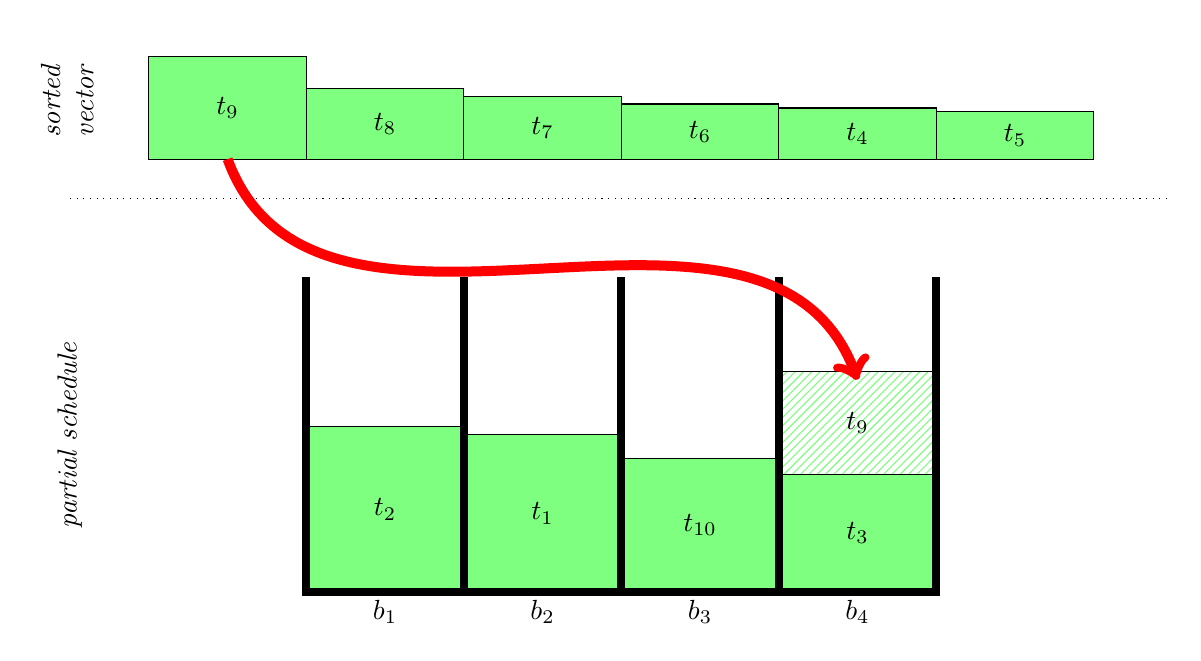
\begin{tikzpicture}
\definecolor{hlearn_bgbox}{RGB}{127,255,127}
\node[shape=rectangle,draw,fill=hlearn_bgbox,minimum width=2cm,minimum height=2.1cm] at (3,1.05) { $t_{2}$ };
\node[shape=rectangle,draw,fill=hlearn_bgbox,minimum width=2cm,minimum height=2.0cm] at (5,1) { $t_{1}$ };
\node[shape=rectangle,draw,fill=hlearn_bgbox,minimum width=2cm,minimum height=1.7cm] at (7,0.85) { $t_{10}$ };
\node[shape=rectangle,draw,fill=hlearn_bgbox,minimum width=2cm,minimum height=1.5cm] at (9,0.75) { $t_{3}$ };

% \node[shape=rectangle,draw,pattern=north east lines,pattern color=hlearn_bgbox,minimum width=2cm,minimum height=1.3cm] at (3,2.75) { $t_{9}$ };
% \node[shape=rectangle,draw,pattern=north east lines,pattern color=hlearn_bgbox,minimum width=2cm,minimum height=1.3cm] at (5,2.65) { $t_{9}$ };
% \node[shape=rectangle,draw,pattern=north east lines,pattern color=hlearn_bgbox,minimum width=2cm,minimum height=1.3cm] at (7,2.35) { $t_{9}$ };
\node[shape=rectangle,draw,pattern=north east lines,pattern color=hlearn_bgbox,minimum width=2cm,minimum height=1.3cm] at (9,2.15) { $t_{9}$ };

\node[shape=rectangle,draw,fill=hlearn_bgbox,minimum width=2cm,minimum height=1.3cm] at (1,0.5+5.65) { $t_{9}$ };
\node[shape=rectangle,draw,fill=hlearn_bgbox,minimum width=2cm,minimum height=0.9cm] at (3,0.5+5.45) { $t_{8}$ };
\node[shape=rectangle,draw,fill=hlearn_bgbox,minimum width=2cm,minimum height=0.8cm] at (5,0.5+5.4) { $t_{7}$ };
\node[shape=rectangle,draw,fill=hlearn_bgbox,minimum width=2cm,minimum height=0.7cm] at (7,0.5+5.35) { $t_{6}$ };
\node[shape=rectangle,draw,fill=hlearn_bgbox,minimum width=2cm,minimum height=0.65cm] at (9,0.5+5.325) { $t_{4}$ };
\node[shape=rectangle,draw,fill=hlearn_bgbox,minimum width=2cm,minimum height=0.6cm] at (11,0.5+5.3) { $t_{5}$ };

% \node at (6,4.5) {\emph{partial schedule}};
% \node at (6,7) {\emph{sorted list}};
\node at (-1,2) {
    \rotatebox{90}{
    \begin{tabular}{c}
    \emph{partial schedule}
%     \emph{partial} \\ \emph{bin packing}
    \end{tabular}
    }};
\node at (-1,6.25) {
    \rotatebox{90}{
    \begin{tabular}{c}
    \emph{sorted} \\ \emph{vector}
    \end{tabular}
%     \emph{sorted vector}
    }};

\draw[dotted] (-1,5) to (13,5);

\draw[line width=0.1cm] (2,4) to (2,0) to (2+2,0) to (2+2,4);
\draw[line width=0.1cm] (4,4) to (4,0) to (4+2,0) to (4+2,4);
\draw[line width=0.1cm] (6,4) to (6,0) to (6+2,0) to (6+2,4);
\draw[line width=0.1cm] (8,4) to (8,0) to (8+2,0) to (8+2,4);

\draw[->,line width=0.05in,color=red] (1,5.5) to [in=110,out=-70] (9,2.7);

\node at (3,-0.25) {$b_1$};
\node at (5,-0.25) {$b_2$};
\node at (7,-0.25) {$b_3$};
\node at (9,-0.25) {$b_4$};
\end{tikzpicture}
\vspace{0.1in}
}
\end{figure}

This conversion process is implemented with the internal function \h{vector2schedule}, whose code is shown in Figure \ref{code:vector2schedule} below.
The details of this function aren't particularly important.
What is important is that \h{vector2schedule} runs in time $\Theta(n\log p)$.
This will be important when determining the run times of the \h{mappend} and \h{train} functions.

\begin{figure}[H]
\caption{The \h{vector2schedule} helper function for LPTF}
\label{code:vector2schedule}
\begin{lstlisting}
vector2schedule :: (Norm a) => Int -> SortedVector a -> Map.Map Int [a]
vector2schedule p vector = snd $ F.foldr cata (emptyheap p,Map.empty) vector
    where
        emptyheap p = Heap.fromAscList [(0,i) | i<-[1..p]]
        cata x (heap,map) = 
            let Just top = Heap.viewHead heap
                set = snd top
                prio = (fst top)+magnitude x
                heap' = Heap.insert (prio,set) (Heap.drop 1 heap)
                map' = Map.insertWith (++) set [x] map
            in (heap',map')

\end{lstlisting}
\end{figure}

Our \h{mappend} operation will implement the LPTF algorithm internally in a way that reuses the results from the input \h{Schedule}s.
We won't be able to reuse the actual schedules, but we can reuse the sorting of the vectors.
We do this by taking advantage of the \h{HomTrainer} instance of the \h{SortedVector} type.
It turns out that merge sort is a monoid homomorphism, and so \h{SortedVector} can be made an instance of the \h{HomTrainer} type class.
The commutative diagram for \h{SortedVector} is shown in Figure \ref{fig:SortedVector} below.

\begin{figure}[H]
\caption{Constructing a \h{SortedVector} is a monoid homomorphism}
\label{fig:SortedVector}
\centering
\begin{tikzpicture}
\draw[->,line width=0.05cm,color=orange] (-1.7in,5.5) to (-1.7in,4.5);
\draw[->,line width=0.05cm,color=orange] (0in,5.5) to (0in,4.5);
\draw[dotted,line width=0.025cm,color=orange] (-1.7in,4.5) to (-1.7in,3.5);
\draw[dotted,line width=0.025cm,color=orange] (0in,4.5) to (0in,3.5);
\draw[->,line width=0.05cm,color=orange] (0in,3.5) to (0in,3) to (2.3in,3) to (2.3in,3.5);
\draw[->,line width=0.05cm,color=orange] (-1.7in,3.5) to (-1.7in,3) to (2.3in,3) to (2.3in,3.5);
\draw[->,line width=0.05cm,color=purple]  (2.3in,5.5) to (2.3in,4.5);
\draw[->,line width=0.05cm,color=purple] (0in,6.5) to (0in,7) to (2.3in,7) to (2.3in,6.5);
\draw[->,line width=0.05cm,color=purple] (-1.7in,6.5) to (-1.7in,7) to (2.3in,7) to (2.3in,6.5);
\draw[dotted,line width=0.025cm,color=purple] (2.3in,6.5) to (2.3in,5.5);

\node at (-1.7in,6) {
    \resizebox{!}{0.25in}{
    \begin{tikzpicture}
    \definecolor{hlearn_bgbox}{RGB}{127,255,127}
    \definecolor{hlearn_bgboxB}{RGB}{224,224,255}
    \node[shape=rectangle,draw,fill=hlearn_bgbox,minimum width=2cm,minimum height=2.1cm]   at (1,1.05) { $t_{a,1}$ };
    \node[shape=rectangle,draw,fill=hlearn_bgbox,minimum width=2cm,minimum height=2.7cm]   at (3,1.35) { $t_{a,2}$ };
    \node[shape=rectangle,draw,fill=hlearn_bgbox,minimum width=2cm,minimum height=3.1cm]   at (5,1.55) { $t_{a,3}$ };;
    \node[shape=rectangle,draw,fill=hlearn_bgbox,minimum width=2cm,minimum height=1.7cm]   at (7,0.85) { $t_{a,4}$ };
    \node[shape=rectangle,draw,fill=hlearn_bgbox,minimum width=2cm,minimum height=1.6cm]   at (9,0.8) { $t_{a,5}$ };
    \node[shape=rectangle,draw,fill=hlearn_bgbox,minimum width=2cm,minimum height=0.6cm]   at (11,0.3) { $t_{a,6}$ };
    \end{tikzpicture}
    }};


\node at (0,6) {
    \resizebox{!}{0.25in}{
%     \resizebox{1.75in}{!}{
    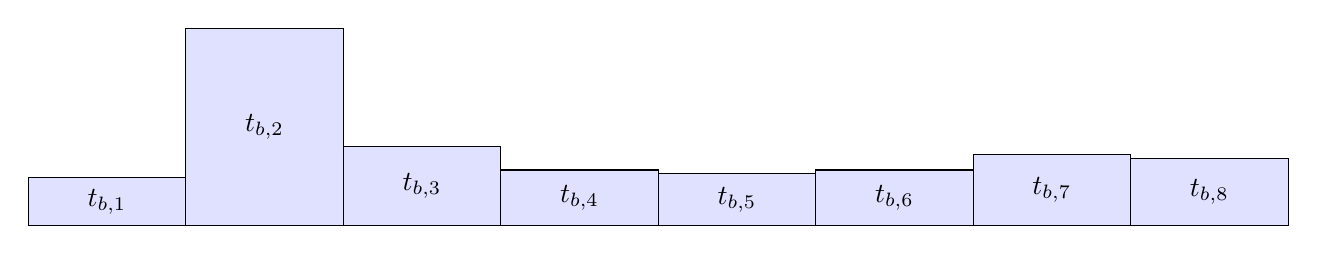
\begin{tikzpicture}
    \definecolor{hlearn_bgbox}{RGB}{127,255,127}
    \definecolor{hlearn_bgboxB}{RGB}{224,224,255}
    \node[shape=rectangle,draw,fill=hlearn_bgboxB,minimum width=2cm,minimum height=0.6cm]  at (1,0.3) { $t_{b,1}$ };
    \node[shape=rectangle,draw,fill=hlearn_bgboxB,minimum width=2cm,minimum height=2.5cm]  at (3,1.25) { $t_{b,2}$ };
    \node[shape=rectangle,draw,fill=hlearn_bgboxB,minimum width=2cm,minimum height=1.0cm]  at (5,0.5) { $t_{b,3}$ };
    \node[shape=rectangle,draw,fill=hlearn_bgboxB,minimum width=2cm,minimum height=0.7cm]  at (7,0.35) { $t_{b,4}$ };
    \node[shape=rectangle,draw,fill=hlearn_bgboxB,minimum width=2cm,minimum height=0.65cm] at (9,0.325) { $t_{b,5}$ };
    \node[shape=rectangle,draw,fill=hlearn_bgboxB,minimum width=2cm,minimum height=0.7cm]  at (11,0.35) { $t_{b,6}$ };
    \node[shape=rectangle,draw,fill=hlearn_bgboxB,minimum width=2cm,minimum height=0.9cm]  at (13,0.45) { $t_{b,7}$ };
    \node[shape=rectangle,draw,fill=hlearn_bgboxB,minimum width=2cm,minimum height=0.85cm] at (15,0.425) { $t_{b,8}$ };
    \end{tikzpicture}
    }};
    
\node at (2.3in,6) {
    \resizebox{!}{0.25in}{
    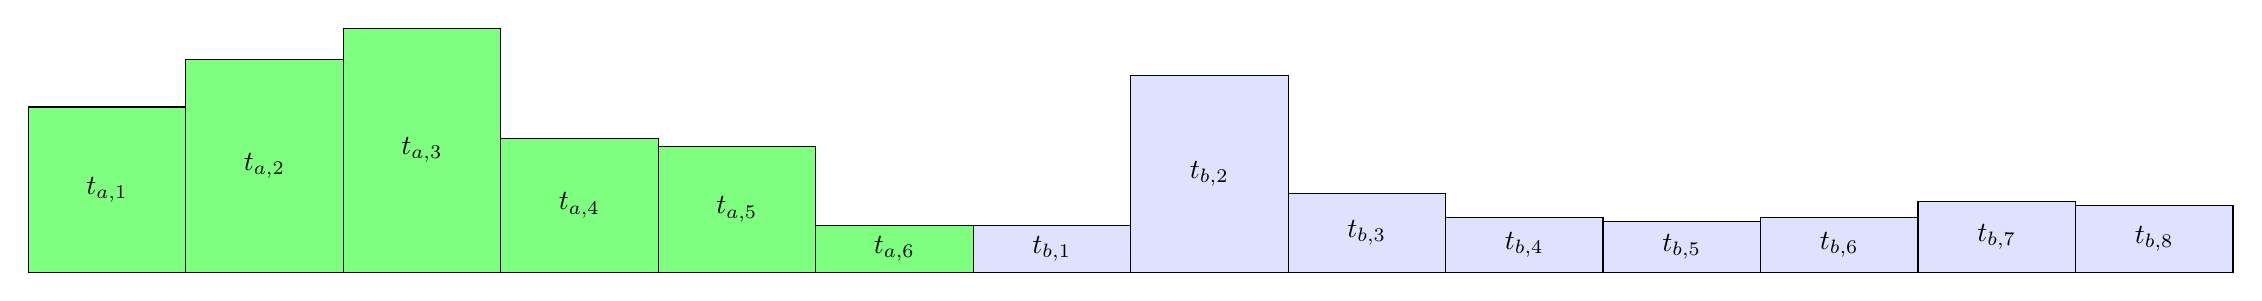
\begin{tikzpicture}
    \definecolor{hlearn_bgbox}{RGB}{127,255,127}
    \definecolor{hlearn_bgboxB}{RGB}{224,224,255}
    \node[shape=rectangle,draw,fill=hlearn_bgbox,minimum width=2cm,minimum height=2.1cm]   at (1,1.05) { $t_{a,1}$ };
    \node[shape=rectangle,draw,fill=hlearn_bgbox,minimum width=2cm,minimum height=2.7cm]   at (3,1.35) { $t_{a,2}$ };
    \node[shape=rectangle,draw,fill=hlearn_bgbox,minimum width=2cm,minimum height=3.1cm]   at (5,1.55) { $t_{a,3}$ };;
    \node[shape=rectangle,draw,fill=hlearn_bgbox,minimum width=2cm,minimum height=1.7cm]   at (7,0.85) { $t_{a,4}$ };
    \node[shape=rectangle,draw,fill=hlearn_bgbox,minimum width=2cm,minimum height=1.6cm]   at (9,0.8) { $t_{a,5}$ };
    \node[shape=rectangle,draw,fill=hlearn_bgbox,minimum width=2cm,minimum height=0.6cm]   at (11,0.3) { $t_{a,6}$ };
    \node[shape=rectangle,draw,fill=hlearn_bgboxB,minimum width=2cm,minimum height=0.6cm]  at (13,0.3) { $t_{b,1}$ };
    \node[shape=rectangle,draw,fill=hlearn_bgboxB,minimum width=2cm,minimum height=2.5cm]  at (15,1.25) { $t_{b,2}$ };
    \node[shape=rectangle,draw,fill=hlearn_bgboxB,minimum width=2cm,minimum height=1.0cm]  at (17,0.5) { $t_{b,3}$ };
    \node[shape=rectangle,draw,fill=hlearn_bgboxB,minimum width=2cm,minimum height=0.7cm]  at (19,0.35) { $t_{b,4}$ };
    \node[shape=rectangle,draw,fill=hlearn_bgboxB,minimum width=2cm,minimum height=0.65cm] at (21,0.325) { $t_{b,5}$ };
    \node[shape=rectangle,draw,fill=hlearn_bgboxB,minimum width=2cm,minimum height=0.7cm]  at (23,0.35) { $t_{b,6}$ };
    \node[shape=rectangle,draw,fill=hlearn_bgboxB,minimum width=2cm,minimum height=0.9cm]  at (25,0.45) { $t_{b,7}$ };
    \node[shape=rectangle,draw,fill=hlearn_bgboxB,minimum width=2cm,minimum height=0.85cm] at (27,0.425) { $t_{b,8}$ };
    \end{tikzpicture}
    }};


\node at (-1.7in,4) {
    \resizebox{!}{0.25in}{
    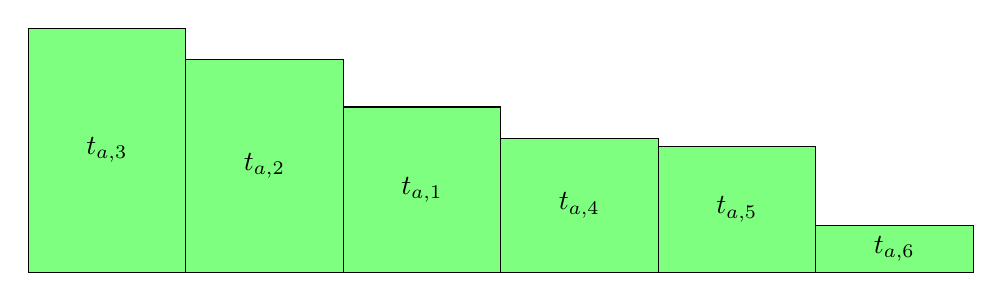
\begin{tikzpicture}
    \definecolor{hlearn_bgbox}{RGB}{127,255,127}
    \definecolor{hlearn_bgboxB}{RGB}{224,224,255}
    \node[shape=rectangle,draw,fill=hlearn_bgbox,minimum width=2cm,minimum height=3.1cm]   at (1,1.55) { $t_{a,3}$ };;
    \node[shape=rectangle,draw,fill=hlearn_bgbox,minimum width=2cm,minimum height=2.7cm]   at (3,1.35) { $t_{a,2}$ };
    \node[shape=rectangle,draw,fill=hlearn_bgbox,minimum width=2cm,minimum height=2.1cm]   at (5,1.05) { $t_{a,1}$ };
    \node[shape=rectangle,draw,fill=hlearn_bgbox,minimum width=2cm,minimum height=1.7cm]   at (7,0.85) { $t_{a,4}$ };
    \node[shape=rectangle,draw,fill=hlearn_bgbox,minimum width=2cm,minimum height=1.6cm]   at (9,0.8) { $t_{a,5}$ };
    \node[shape=rectangle,draw,fill=hlearn_bgbox,minimum width=2cm,minimum height=0.6cm]   at (11,0.3) { $t_{a,6}$ };
    \end{tikzpicture}
    }};

% \node at (-2.5in,0) {
%     \resizebox{1.5in}{!}{
%     \begin{tikzpicture}
%     \definecolor{hlearn_bgbox}{RGB}{127,255,127}
%     \node[shape=rectangle,draw,fill=hlearn_bgbox,minimum width=2cm,minimum height=3.1cm] at (3,1.55) { $t_{a,3}$ };
%     \node[shape=rectangle,draw,fill=hlearn_bgbox,minimum width=2cm,minimum height=0.6cm] at (3,3.4) { $t_{a,6}$ };
%     \node[shape=rectangle,draw,fill=hlearn_bgbox,minimum width=2cm,minimum height=2.7cm] at (5,1.35) { $t_{a,2}$ };
%     \node[shape=rectangle,draw,fill=hlearn_bgbox,minimum width=2cm,minimum height=1.6cm] at (5,3.5) { $t_{a,5}$ };
%     \node[shape=rectangle,draw,fill=hlearn_bgbox,minimum width=2cm,minimum height=2.1cm] at (7,1.05) { $t_{a,1}$ };
%     \node[shape=rectangle,draw,fill=hlearn_bgbox,minimum width=2cm,minimum height=1.7cm] at (7,2.95) { $t_{a,4}$ };
%     \draw[line width=0.1cm] (2,7.0) to (2,0) to (2+2,0) to (2+2,7.0);
%     \draw[line width=0.1cm] (4,7.0) to (4,0) to (4+2,0) to (4+2,7.0);
%     \draw[line width=0.1cm] (6,7.0) to (6,0) to (6+2,0) to (6+2,7.0);
%     \node at (3,-0.5) {$b_{1}$};
%     \node at (5,-0.5) {$b_{2}$};
%     \node at (7,-0.5) {$b_{3}$};
%     \end{tikzpicture}
%     }};

\node at (0,4) {
    \resizebox{!}{0.25in}{
    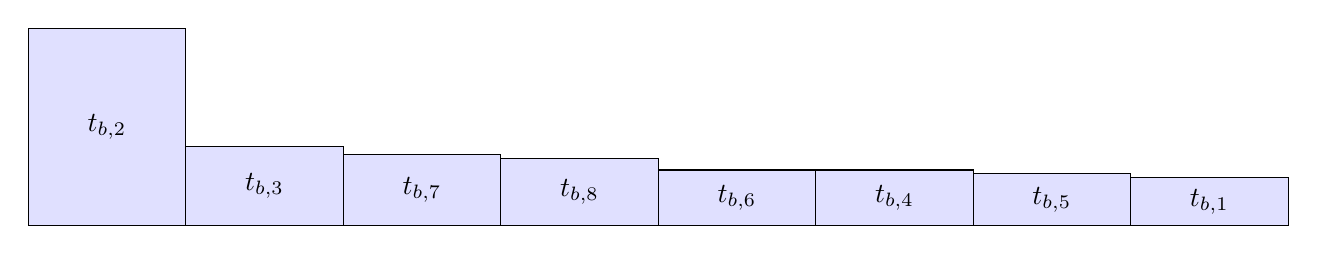
\begin{tikzpicture}
    \definecolor{hlearn_bgbox}{RGB}{127,255,127}
    \definecolor{hlearn_bgboxB}{RGB}{224,224,255}
    \node[shape=rectangle,draw,fill=hlearn_bgboxB,minimum width=2cm,minimum height=2.5cm]  at (1,1.25) { $t_{b,2}$ };
    \node[shape=rectangle,draw,fill=hlearn_bgboxB,minimum width=2cm,minimum height=1.0cm]  at (3,0.5) { $t_{b,3}$ };
    \node[shape=rectangle,draw,fill=hlearn_bgboxB,minimum width=2cm,minimum height=0.9cm]  at (5,0.45) { $t_{b,7}$ };
    \node[shape=rectangle,draw,fill=hlearn_bgboxB,minimum width=2cm,minimum height=0.85cm] at (7,0.425) { $t_{b,8}$ };
    \node[shape=rectangle,draw,fill=hlearn_bgboxB,minimum width=2cm,minimum height=0.7cm]  at (9,0.35) { $t_{b,6}$ };
    \node[shape=rectangle,draw,fill=hlearn_bgboxB,minimum width=2cm,minimum height=0.7cm]  at (11,0.35) { $t_{b,4}$ };
    \node[shape=rectangle,draw,fill=hlearn_bgboxB,minimum width=2cm,minimum height=0.65cm] at (13,0.325) { $t_{b,5}$ };
    \node[shape=rectangle,draw,fill=hlearn_bgboxB,minimum width=2cm,minimum height=0.6cm]  at (15,0.3) { $t_{b,1}$ };
    \end{tikzpicture}
    }};

% \node at (0.5,0) {
%     \resizebox{1.5in}{!}{
%     \begin{tikzpicture}
%     \definecolor{hlearn_bgboxB}{RGB}{224,224,255}
%     \node[shape=rectangle,draw,fill=hlearn_bgboxB,minimum width=2cm,minimum height=2.5cm] at (3,1.25) { $t_{b,2}$ };
%     \node[shape=rectangle,draw,fill=hlearn_bgboxB,minimum width=2cm,minimum height=1.0cm] at (5,0.5) { $t_{b,3}$ };
%     \node[shape=rectangle,draw,fill=hlearn_bgboxB,minimum width=2cm,minimum height=0.7cm] at (5,1.35) { $t_{b,4}$ };
%     \node[shape=rectangle,draw,fill=hlearn_bgboxB,minimum width=2cm,minimum height=0.7cm] at (5,2.05) { $t_{b,6}$ };
%     \node[shape=rectangle,draw,fill=hlearn_bgboxB,minimum width=2cm,minimum height=0.6cm] at (5,2.6999999999999997) { $t_{b,1}$ };
%     \node[shape=rectangle,draw,fill=hlearn_bgboxB,minimum width=2cm,minimum height=0.9cm] at (7,0.45) { $t_{b,7}$ };
%     \node[shape=rectangle,draw,fill=hlearn_bgboxB,minimum width=2cm,minimum height=0.85cm] at (7,1.325) { $t_{b,8}$ };
%     \node[shape=rectangle,draw,fill=hlearn_bgboxB,minimum width=2cm,minimum height=0.65cm] at (7,2.075) { $t_{b,5}$ };
%     \draw[line width=0.1cm] (2,7.0) to (2,0) to (2+2,0) to (2+2,7.0);
%     \draw[line width=0.1cm] (4,7.0) to (4,0) to (4+2,0) to (4+2,7.0);
%     \draw[line width=0.1cm] (6,7.0) to (6,0) to (6+2,0) to (6+2,7.0);
%     \node at (3,-0.5) {$b_{1}$};
%     \node at (5,-0.5) {$b_{2}$};
%     \node at (7,-0.5) {$b_{3}$};
%     \end{tikzpicture}
%     }};

\node at (2.3in,4) {
    \resizebox{!}{0.25in}{
    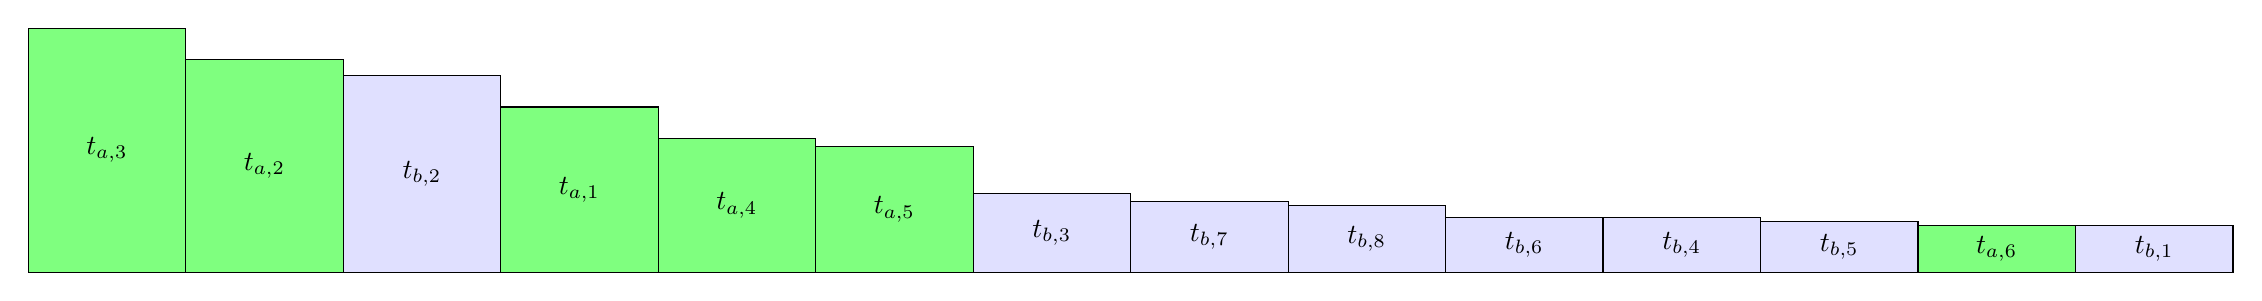
\begin{tikzpicture}
    \definecolor{hlearn_bgbox}{RGB}{127,255,127}
    \definecolor{hlearn_bgboxB}{RGB}{224,224,255}
    \node[shape=rectangle,draw,fill=hlearn_bgbox,minimum width=2cm,minimum height=3.1cm]   at (1,1.55) { $t_{a,3}$ };;
    \node[shape=rectangle,draw,fill=hlearn_bgbox,minimum width=2cm,minimum height=2.7cm]   at (3,1.35) { $t_{a,2}$ };
    \node[shape=rectangle,draw,fill=hlearn_bgboxB,minimum width=2cm,minimum height=2.5cm]  at (5,1.25) { $t_{b,2}$ };
    \node[shape=rectangle,draw,fill=hlearn_bgbox,minimum width=2cm,minimum height=2.1cm]   at (7,1.05) { $t_{a,1}$ };
    \node[shape=rectangle,draw,fill=hlearn_bgbox,minimum width=2cm,minimum height=1.7cm]   at (9,0.85) { $t_{a,4}$ };
    \node[shape=rectangle,draw,fill=hlearn_bgbox,minimum width=2cm,minimum height=1.6cm]   at (11,0.8) { $t_{a,5}$ };
    \node[shape=rectangle,draw,fill=hlearn_bgboxB,minimum width=2cm,minimum height=1.0cm]  at (13,0.5) { $t_{b,3}$ };
    \node[shape=rectangle,draw,fill=hlearn_bgboxB,minimum width=2cm,minimum height=0.9cm]  at (15,0.45) { $t_{b,7}$ };
    \node[shape=rectangle,draw,fill=hlearn_bgboxB,minimum width=2cm,minimum height=0.85cm] at (17,0.425) { $t_{b,8}$ };
    \node[shape=rectangle,draw,fill=hlearn_bgboxB,minimum width=2cm,minimum height=0.7cm]  at (19,0.35) { $t_{b,6}$ };
    \node[shape=rectangle,draw,fill=hlearn_bgboxB,minimum width=2cm,minimum height=0.7cm]  at (21,0.35) { $t_{b,4}$ };
    \node[shape=rectangle,draw,fill=hlearn_bgboxB,minimum width=2cm,minimum height=0.65cm] at (23,0.325) { $t_{b,5}$ };
    \node[shape=rectangle,draw,fill=hlearn_bgbox,minimum width=2cm,minimum height=0.6cm]   at (25,0.3) { $t_{a,6}$ };
    \node[shape=rectangle,draw,fill=hlearn_bgboxB,minimum width=2cm,minimum height=0.6cm]  at (27,0.3) { $t_{b,1}$ };
    \end{tikzpicture}
    }};
    
% \node at (-1in,-8) {
%     \resizebox{1.5in}{!}{
%     \begin{tikzpicture}
%     \definecolor{hlearn_bgbox}{RGB}{127,255,127}
%     \definecolor{hlearn_bgboxB}{RGB}{224,224,255}
%     \node[shape=rectangle,draw,fill=hlearn_bgbox,minimum width=2cm,minimum height=3.1cm] at (3,1.55) { $t_{a,3}$ };
%     \node[shape=rectangle,draw,fill=hlearn_bgbox,minimum width=2cm,minimum height=1.6cm] at (3,3.9000000000000004) { $t_{a,5}$ };
%     \node[shape=rectangle,draw,fill=hlearn_bgboxB,minimum width=2cm,minimum height=0.85cm] at (3,5.125) { $t_{b,8}$ };
%     \node[shape=rectangle,draw,fill=hlearn_bgboxB,minimum width=2cm,minimum height=0.65cm] at (3,5.875) { $t_{b,5}$ };
%     \node[shape=rectangle,draw,fill=hlearn_bgbox,minimum width=2cm,minimum height=2.7cm] at (5,1.35) { $t_{a,2}$ };
%     \node[shape=rectangle,draw,fill=hlearn_bgbox,minimum width=2cm,minimum height=1.7cm] at (5,3.5500000000000003) { $t_{a,4}$ };
%     \node[shape=rectangle,draw,fill=hlearn_bgboxB,minimum width=2cm,minimum height=1.0cm] at (5,4.9) { $t_{b,3}$ };
%     \node[shape=rectangle,draw,fill=hlearn_bgboxB,minimum width=2cm,minimum height=0.7cm] at (5,5.75) { $t_{b,4}$ };
%     \node[shape=rectangle,draw,fill=hlearn_bgbox,minimum width=2cm,minimum height=0.6cm] at (5,6.4) { $t_{a,6}$ };
%     \node[shape=rectangle,draw,fill=hlearn_bgboxB,minimum width=2cm,minimum height=2.5cm] at (7,1.25) { $t_{b,2}$ };
%     \node[shape=rectangle,draw,fill=hlearn_bgbox,minimum width=2cm,minimum height=2.1cm] at (7,3.55) { $t_{a,1}$ };
%     \node[shape=rectangle,draw,fill=hlearn_bgboxB,minimum width=2cm,minimum height=0.9cm] at (7,5.05) { $t_{b,7}$ };
%     \node[shape=rectangle,draw,fill=hlearn_bgboxB,minimum width=2cm,minimum height=0.7cm] at (7,5.85) { $t_{b,6}$ };
%     \node[shape=rectangle,draw,fill=hlearn_bgboxB,minimum width=2cm,minimum height=0.6cm] at (7,6.5) { $t_{b,1}$ };
%     \draw[line width=0.1cm] (2,7.0) to (2,0) to (2+2,0) to (2+2,7.0);
%     \draw[line width=0.1cm] (4,7.0) to (4,0) to (4+2,0) to (4+2,7.0);
%     \draw[line width=0.1cm] (6,7.0) to (6,0) to (6+2,0) to (6+2,7.0);
%     \node at (3,-0.5) {$b_{1}$};
%     \node at (5,-0.5) {$b_{2}$};
%     \node at (7,-0.5) {$b_{3}$};
%     \end{tikzpicture}
%     }};

\node at (-1in,4) {$\diamond$};
\node at (-1in,6) {$\diamond$};
\node at (1in,4) {$=$};
\node at (1in,6) {$=$};

\draw[dotted] (-2in,5) to (3in,5);

\end{tikzpicture}
\vspace{.15in}
\end{figure}

It is important to note that \h{SortedVector}'s \h{mappend} operation does not take constant time.
In fact, it takes $\Theta(n)$ time, where $n$ is the size of both input vectors put together.
The \h{HomTrainer} type class can handle these non-constant \h{mappend} operations elegantly.
By looking up in Table \ref{table:rt}, we can see the run times of the derived algorithms.
Notice that if the monoid operation takes time $\Theta(n)$, then our batch trainer will take time $\Theta(n\log n)$, and this is exactly what we would expect for a sorting.
Details of how these numbers were derived can be found in my TFP13 submission on the HLearn library \cite{me_tfp13}.

\begin{table}[H]
\caption{Given a run time for \h{mappend}, you can calculate the run time of the automatically generated functions using this table.}
\label{table:rt}
% \centering
\hspace{-0.3in}
\begin{tabular}{ c | c | c | c}
\hline
Monoid operation & Sequential batch trainer & \ \ Parallel batch trainer\ \ & Online trainer\\
\mbox{(\h{mapend})} & \mbox{(\h{train})} & \mbox{(\h{parallel train})} & \mbox{(\h{add1dp})}\\
\hline \hline
$\Theta(1)$ & $\Theta(n)$ & $\Theta\left(\frac{n}{p}+\log p\right)$ & $\Theta(1)$ \\
$\Theta(\log^a n)$, $a>0$ & $\Theta(n)$ & $\Theta\left(\frac{n}{p}+(\log^a n)(\log p)\right)$ & $\Theta(\log^a n)$ \\
$\Theta(n)$ & $\Theta(n\log n)$ & $\Theta\left(\frac{n}{p}\log\frac{n}{p}+n\right)$ & $\Theta(n)$ \\
$\Theta(n^b)$, $b>1$ & $\Theta(n^b)$ & no improvement & no improvement\\
\hline
\end{tabular}
\end{table}

% We're now ready to look at the \h{Monoid} instance for \h{Scheduling}.
With all of these building blocks in place, the \h{Monoid} instance for \h{Scheduling} is relatively simple.
The \h{mempty} and \h{mappend} operations are exactly the same as they are for \h{SortedVector}, except that we also call the helper function \h{lptf}.
This function just packages the \h{SortedVector} into a \h{Scheduling} type using the \h{vector2schedule} function we saw earlier.
\begin{figure}[H]
\begin{lstlisting}
instance (Ord a, Norm a, SingI n) => Monoid (Scheduling n a) where
    mempty = lptf mempty
    p1 `mappend` p2 = lptf $ (vector p1) <> (vector p2)
    
lptf :: forall a p. (Norm a, SingI p) => SortedVector a -> Scheduling p a
lptf vector = Scheduling
    { vector = vector
    , schedule = vector2schedule p vector
    }
    where p = fromIntegral $ fromSing (sing :: Sing n))
\end{lstlisting}
\caption{The \h{Monoid} instance for the \h{Scheduling} model}
\end{figure}
Since \h{vector2schedule} runs in linear time and \h{SortedVector}'s \h{mappend} runs in linear time, the \h{Scheduling}'s \h{mappend} runs in linear time as well.
By Table \ref{table:rt} again, we have that the automatically derived batch trainer will take time $\Theta(n\log n)$.
This is exactly what the traditional LPTF algorithm takes.

Of course, we still have to implement the \h{HomTrainer} instance.
But this is easy.
Inside the \h{HomTrainer} class is a function called the ``singleton trainer'':
\begin{spec}
train1dp :: HomTrainer model => Datapoint model -> model
\end{spec}
All this function does is create a model from a single data point.\footnote{The \h{train1dp} function is analogous to the \h{pure} function in the \h{Applicative} class, or the \h{return} function in the \h{Monad} class.}
In practice, such a singleton model is rarely useful by itself.
But if we define it, then the compiler can then use this function and \h{mappend} to build the other functions within the \h{HomTrainer} class automatically.
This is how we get the online and parallel functions ``for free.''

The resulting \h{Scheduling} instance looks like:
\begin{figure}[H]
\begin{lstlisting}
instance (Norm a, SingI n) => HomTrainer (Scheduling n a) where
    type Datapoint (Scheduling n a) = a
    train1dp dp = lptf $ train1dp dp
\end{lstlisting}
\caption{The \h{HomTrainer} instance is quite short and mechanical to write}
\end{figure}
That's all we \textit{need} to do to guarantee correct asymptotic performance, but we've got one last trick that will speed up our \h{train} function by a constant factor.
Recall that when performing the \h{mappend} operation on \h{Scheduling} variables, we can only reuse the work contained inside of \h{vector}.
The old \h{schedule}s must be completely discarded.
Since \h{mappend} is called many times in our automatically generated functions, calculating all of these intermediate schedules would give us no benefit but result in a lot of extra work.
That is why in the \h{Scheduling} type, the \h{vector} member was declared strict, whereas the \h{schedule} member was declared lazy.
The \h{schedule}s won't actually be calculated until someone demands them, and since no one will ever demand a schedule from the intermediate steps, we never calculate them.

\section{Back to Bin Packing}

Since \prob{BinPacking} and \prob{Scheduling} were such similar problems, it's not too surprising that a similar technique can be used to implement a \h{BinPacking} model.
% We can solving \prob{BinPacking} will look similar to how we solved \prob{Scheduling}.
% We can approximately solve a \prob{BinPacking} problem similarly to how we derived a Scheduling instance.
The main difference is that we'll replace the LPTF algorithm with another simple algorithm called Best Fit Decreasing (BFD).  This gives us the performance guarantee of:
$$
\textit{BFD} \le {11\over9}\textit{OPT} + 1
$$
There are some slightly better approximations for \prob{BinPacking}, but we won't look at them here because they are much more complicated.
Chapter 2 of \textit{Approximation Algorithms for NP Hard Problems} gives a good overview on the considerable amount of literature for bin packing \cite{hochbaum96binpacking}.

BFD is a two stage algorithm in the same vein as LPTF.
First, we sort the data points by size.
% This step dominates our run time, so our batch trainer will run in time $\Theta(n\log n)$ and our monoid operation in time $\Theta(n)$.
Then, we iteratively take the largest item and find the ``best'' bin to place it in.
The best bin is defined as the bin with the least amount of space that can still hold the item.
If no bins can hold the item, then we create a new bin and add the item there.
This is shown graphically in Figure \ref{fig:bfd} below.

\begin{figure}[H]
\caption{One iteration of the Best First Decreasing (BFD) algorithm}
\label{fig:bfd}
\centering
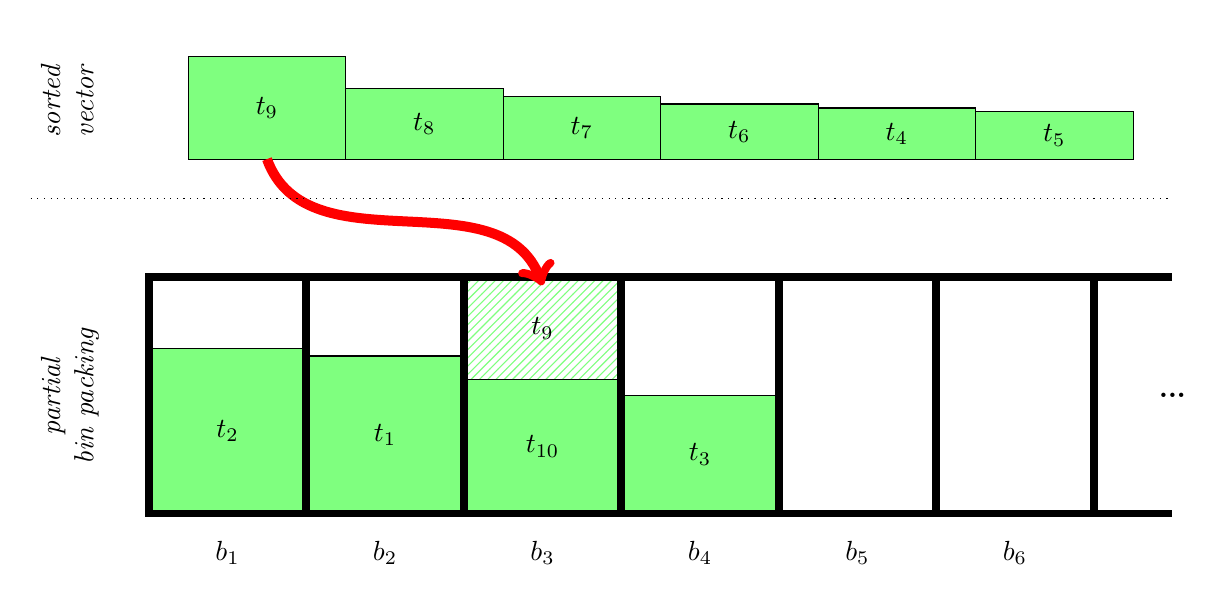
\begin{tikzpicture}
    \definecolor{hlearn_bgbox}{RGB}{127,255,127}
%     \node[shape=rectangle,draw,fill=hlearn_bgbox,minimum width=2cm,minimum height=2.1cm] at (1,1.05) { $t_{2}$ };
%     \node[shape=rectangle,draw,fill=hlearn_bgbox,minimum width=2cm,minimum height=2.0cm] at (3,1.0) { $t_{1}$ };
%     \node[shape=rectangle,draw,fill=hlearn_bgbox,minimum width=2cm,minimum height=1.7cm] at (5,0.85) { $t_{10}$ };
%     \node[shape=rectangle,draw,fill=hlearn_bgbox,minimum width=2cm,minimum height=1.5cm] at (7,0.75) { $t_{3}$ };
    \node[shape=rectangle,draw,fill=hlearn_bgbox,minimum width=2cm,minimum height=1.3cm] at (3.5,0.5+4.65) { $t_{9}$ };
    \node[shape=rectangle,draw,fill=hlearn_bgbox,minimum width=2cm,minimum height=0.9cm] at (5.5,0.5+4.45) { $t_{8}$ };
    \node[shape=rectangle,draw,fill=hlearn_bgbox,minimum width=2cm,minimum height=0.8cm] at (7.5,0.5+4.4) { $t_{7}$ };
    \node[shape=rectangle,draw,fill=hlearn_bgbox,minimum width=2cm,minimum height=0.7cm] at (9.5,0.5+4.35) { $t_{6}$ };
    \node[shape=rectangle,draw,fill=hlearn_bgbox,minimum width=2cm,minimum height=0.65cm] at (11.5,0.5+4.325) { $t_{4}$ };
    \node[shape=rectangle,draw,fill=hlearn_bgbox,minimum width=2cm,minimum height=0.6cm] at (13.5,0.5+4.3) { $t_{5}$ };

    \definecolor{hlearn_bgbox}{RGB}{127,255,127}
    \definecolor{hlearn_bgbox_tmp}{RGB}{223,255,223}
%     \definecolor{hlearn_bgbox_tmp}{RGB}{127,255,127}
    \node[shape=rectangle,draw,fill=hlearn_bgbox,minimum width=2cm,minimum height=2.1cm] at (3,1.05) { $t_{2}$ };
%     \node[shape=rectangle,draw,fill=hlearn_bgbox,minimum width=2cm,minimum height=0.7cm] at (3,2.45) { $t_{6}$ };
    \node[shape=rectangle,draw,fill=hlearn_bgbox,minimum width=2cm,minimum height=2.0cm] at (5,1.0) { $t_{1}$ };
%     \node[shape=rectangle,draw,fill=hlearn_bgbox,minimum width=2cm,minimum height=0.8cm] at (5,2.4) { $t_{7}$ };
    \node[shape=rectangle,draw,fill=hlearn_bgbox,minimum width=2cm,minimum height=1.7cm] at (7,0.85) { $t_{10}$ };
%     \node[shape=rectangle,draw,fill=hlearn_bgbox,minimum width=2cm,minimum height=0.9cm] at (7,2.15) { $t_{8}$ };
    \node[shape=rectangle,draw,fill=hlearn_bgbox,minimum width=2cm,minimum height=1.5cm] at (9,0.75) { $t_{3}$ };
%     \node[shape=rectangle,draw,fill=hlearn_bgbox,minimum width=2cm,minimum height=0.65cm] at (11,0.325) { $t_{4}$ };
%     \node[shape=rectangle,draw,fill=hlearn_bgbox,minimum width=2cm,minimum height=0.6cm] at (11,0.95) { $t_{5}$ };

%     \node[shape=rectangle,pattern=north east lines,pattern color=hlearn_bgbox,draw,minimum width=2cm,minimum height=1.3cm] at (3,2.75) { $t_{9}$ };
%     \node[shape=rectangle,pattern=north east lines,pattern color=hlearn_bgbox,draw,minimum width=2cm,minimum height=1.3cm] at (5,2.65) { $t_{9}$ };
    \node[shape=rectangle,pattern=north east lines,pattern color=hlearn_bgbox,draw,minimum width=2cm,minimum height=1.3cm] at (7,2.35) { $t_{9}$ };
%     \node[shape=rectangle,pattern=north east lines,pattern color=hlearn_bgbox,draw,minimum width=2cm,minimum height=1.3cm] at (9,2.15) { $t_{9}$ };
%     \node[shape=rectangle,pattern=north east lines,pattern color=hlearn_bgbox,draw,minimum width=2cm,minimum height=1.3cm] at (11,0.65) { $t_{9}$ };

    \draw[line width=0.1cm] (2,3.0) to (2,0) to (2+2,0) to (2+2,3.0);
    \draw[line width=0.1cm] (4,3.0) to (4,0) to (4+2,0) to (4+2,3.0);
    \draw[line width=0.1cm] (6,3.0) to (6,0) to (6+2,0) to (6+2,3.0);
    \draw[line width=0.1cm] (8,3.0) to (8,0) to (8+2,0) to (8+2,3.0);
    \draw[line width=0.1cm] (10,3.0) to (10,0) to (10+2,0) to (10+2,3.0);
    \draw[line width=0.1cm] (12,3.0) to (12,0) to (12+2,0) to (12+2,3.0);

    \node at (3,-0.5) {$b_{1}$};
    \node at (5,-0.5) {$b_{2}$};
    \node at (7,-0.5) {$b_{3}$};
    \node at (9,-0.5) {$b_{4}$};
    \node at (11,-0.5) {$b_{5}$};
    \node at (13,-0.5) {$b_{6}$};
    % \draw[line width=0.1cm] (14,3.0) to (14,0) to node[below] {$b_{5}$} (14+2,0) to (14+2,3.0);
    % \draw[line width=0.1cm] (16,3.0) to (16,0) to node[below] {$b_{5}$} (16+2,0) to (16+2,3.0);
    \draw[line width=0.1cm] (2,0) to (2,3.0) to (15,3.0);
    \draw[line width=0.1cm] (2,0) to (15,0);
    % \draw[dashed,color=red,line width=0.05cm] (2,3) to (2,4);
    % \draw[dashed,color=red,line width=0.05cm] (12,3) to (12,4);
    % \draw[<->,line width=0.05cm,color=red] (2,3.5) to node[above] {number of bins} (12,3.5);
    % \draw[<->,line width=0.05cm,color=blue] (1.5,0) to (1.5,3);
    % \draw[dashed,color=blue,line width=0.05cm] (1,0) to (2,0);
    % \draw[dashed,color=blue,line width=0.05cm] (1,3) to (2,3);
    % \node[color=blue] at (1,1.5) {\rotatebox{90}{fixed bin size}};
    \node at (15,1.5) {\textbf{...}};

    \draw[->,line width=0.05in,color=red] (3.5,4.5) to [in=110,out=-70] (7,2.9);

    \draw[dotted] (0.5,4) to (15,4);
    
\node at (1,1.5) {
    \rotatebox{90}{
    \begin{tabular}{c}
    \emph{partial} \\ \emph{bin packing}
    \end{tabular}
    }};
% \node[text centered] at (0,1.5) {\emph{partial \\ bin packing}};
\node at (1,5.25) {
    \rotatebox{90}{
    \begin{tabular}{c}
    \emph{sorted} \\ \emph{vector}
    \end{tabular}
%     \emph{sorted vector}
    }};

\end{tikzpicture}
\vspace{0.05in}
\end{figure}

The data type for bin packing is:
\begin{spec}
data BinPacking (n::Nat) a = BinPacking
    { vector  :: !(SortedVector a)
    , packing :: Map.Map Bin [a]
    }
\end{spec}
This is the exact same form as the Scheduling type had.
The only difference is that we will use the BFD strategy to generate our \h{Map}.
Therefore, by similar reasoning, the \h{BinPacking}'s \h{mappend} function takes time $\Theta(n)$ and its \h{train} function takes time $\Theta(n\log n)$.
Again, this is exactly what the traditional description of the BFD algorithm requires.

\section{Takeaways}

Most instances of the \h{HomTrainer} type class are related to statistics or machine learning, but the class is much more general than that.
For example, we've just seen how to use \h{HomTrainer}s to approximate two \np-complete problems.
So from now on, whenever you see a function that has type:
\begin{spec}
 :: [datapoint] -> model
\end{spec}
ask yourself, ``Could this algorithm be implemented using a \h{HomTrainer}?''
If yes, you'll get online and parallel versions for free.

Finally, we've looked at the monoid structure for \h{Scheduling} and \h{BinPacking}, but these types also have Abelian group and $\mathbb{Z}$-module structure as well.
I'll let you explore the documentation available on the github repository \cite{hlearn} 
(pull requests are always welcome!)
to find creative ways to exploit these structures.
If you have any questions or feedback, I'd love to hear it.

% \bibliographystyle{plain}
\bibliography{bibliography}

\end{document}